\documentclass[sr]{drdc-report}
\usepackage[pdfa,pdfpagemode={UseOutlines},bookmarks=true,bookmarksopen=true,bookmarksopenlevel=0,bookmarksnumbered=true,hypertexnames=false,colorlinks,linkcolor={black},citecolor={black},urlcolor={black},pdfstartview={FitV},linktoc={all},breaklinks=true,pagebackref=false]{hyperref}
%\usepackage{drdc-distlist}
 \usepackage{drdc-docctl}
% \usepackage[T1]{fontenc}
 \usepackage[utf8]{inputenc}
 \usepackage[tbtags]{amsmath} %Tags at the bottom for multi-lines
 \usepackage{amssymb}
 \usepackage{mathtools}
 \usepackage{graphicx}
 \usepackage{booktabs}
 \usepackage{dcolumn}
 \usepackage{longtable}
 \usepackage[pdf]{pstricks}
 \usepackage{pst-node}
 \usepackage{pst-blur}
% \usepackage{auto-pst-pdf}
 \usepackage{afterpage}
 \usepackage[toc,page]{appendix}
 \usepackage{subfig}
% \usepackage[lite,subscriptcorrection,nofontinfo]{mtpro2}
 \makeatletter
 \newcommand\tm{\ensuremath{{}^\text{TM}}}
 \makeatother
 \DeclarePairedDelimiter{\floor}{\lfloor}{\rfloor}

\def\tvec{\ensuremath{\vec{\theta}}}
\def\pvec{\ensuremath{\vec{\phi}}}

\def\Eqref#1{Equation~\eqref{#1}}
\def\relabel#1{\tag{\ref{#1}}}

\def\f#1{\ensuremath{f\left(#1\right)}}
\def\fc#1#2{{\newbox\fvars\setbox\fvars=\hbox{\ensuremath{#1}}\newdimen\fvarsh\fvarsh=\ht\fvars\ensuremath{f\left(\box\fvars\left|\vrule height\fvarsh width0pt{#2}\right.\right)}}}
\def\P#1{\ensuremath{P\left(#1\right)}}
\def\Pc#1#2{{\newbox\fvars\setbox\fvars=\hbox{\ensuremath{#1}}\newdimen\fvarsh\fvarsh=\ht\fvars\ensuremath{P\left(\box\fvars\left|\vrule height\fvarsh width0pt{#2}\right.\right)}}}
\def\f#1{\ensuremath{f\left(#1\right)}}
\def\fc#1#2{{\newbox\fvars\setbox\fvars=\hbox{\ensuremath{#1}}\newdimen\fvarsh\fvarsh=\ht\fvars\ensuremath{f\left(\box\fvars\left|\vrule height\fvarsh width0pt{#2}\right.\right)}}}
\def\Lc#1#2{{\newbox\fvars\setbox\fvars=\hbox{\ensuremath{#1}}\newdimen\fvarsh\fvarsh=\ht\fvars\ensuremath{L\left(\box\fvars\left|\vrule height\fvarsh width0pt{#2}\right.\right)}}}

\def\Rz{\ensuremath{R_0}}
\def\Reff{\ensuremath{R_\mathrm{eff}}}
\def\Robs{\ensuremath{R_\mathrm{obs}}}
\def\Pinf{\ensuremath{P_\mathrm{inf}}}
\def\Pt{\ensuremath{P_\mathrm{t}}}
\def\ttpr{\ensuremath{t_\mathrm{t.p.r.}}}
\def\mtpr{\ensuremath{m_\mathrm{t.p.r.}}}
\def\tdeltat{\ensuremath{T_{\Delta t}}}
\def\ctwindow{\ensuremath{\texttt{ctwindow}}}
\def\Pit{\ensuremath{P_{{\hspace{0.25em}}^\mathrm{i}t}}}
\def\Pim{\ensuremath{P_{{\hspace{0.25em}}^\mathrm{i}m}}}
\def\imbar{\ensuremath{{}^\textrm{i}\bar{m}}}
\def\itbar{\ensuremath{{}^\textrm{i}\bar{t}}}
\def\npaths{\ensuremath{n_\textrm{paths}}}
\def\tmax{\ensuremath{t_\textrm{max}}}
\def\grouplog{\texttt{group\_log}}
\def\timerelpriendcomm{\texttt{time\_rel\_pri\_end\_comm}}
\def\observablepathsonly{\texttt{observable\_paths\_only}}
\def\prinoaltperiod{\texttt{pri\_no\_alt\_period}}
\def\prinomainperiod{\texttt{pri\_no\_main\_period}}

\def\nfpc{\ensuremath{95^\mathrm{th}}}

\newcommand{\Tau}{\mathcal{T}}

\newcommand{\Nt}{\ensuremath{{\mathcal{N}_\mathrm{t}(\tau_i)}}}
\newcommand{\Ntfixed}{\ensuremath{{\mathcal{N}_\mathrm{t}}}}
\newcommand{\Nti}{\ensuremath{{\mathcal{N}_\mathrm{i}(\tau_i)}}}
\newcommand{\Ntifixed}{\ensuremath{{\mathcal{N}_\mathrm{i}}}}
\newcommand{\Nts}{\ensuremath{{\mathcal{N}_\mathrm{s}(\tau_i)}}}
\newcommand{\Ntsfixed}{\ensuremath{{\mathcal{N}_\mathrm{s}}}}
\newcommand{\Ntvar}{\ensuremath{{\mathcal{N}_\mathrm{t}(\tau)}}}
\newcommand{\Ntivar}{\ensuremath{{\mathcal{N}_\mathrm{i}(\tau)}}}
\newcommand{\Ntsvar}{\ensuremath{{\mathcal{N}_\mathrm{s}(\tau)}}}
\newcommand{\pinf}{\ensuremath{{p_\mathrm{i}(\tau_i)}}}
\newcommand{\Yi}{\ensuremath{{Y(\tau_i)}}}
\newcommand{\Ni}{\ensuremath{{N_\mathrm{i}}}}
\newcommand{\Ns}{\ensuremath{{N_\mathrm{s}}}}
\renewcommand{\ni}{\ensuremath{{n_\mathrm{i}}}}
\newcommand{\ns}{\ensuremath{{n_\mathrm{s}}}}
\newcommand{\Da}{\ensuremath{{\prescript{\alpha}{}{\!D}}}}
\newcommand{\Db}{\ensuremath{{\prescript{\beta}{}{\!D}}}}
\newcommand{\Fa}{\ensuremath{{\prescript{\alpha}{}{\!\mathcal{F}}}}}
\newcommand{\Fb}{\ensuremath{{\prescript{\beta}{}{\!\mathcal{F}}}}}
\newcommand{\Yia}{\ensuremath{{\prescript{\alpha}{}{\!\Yi}}}}
\newcommand{\Yib}{\ensuremath{{\prescript{\beta}{}{\!\Yi}}}}
\newcommand{\Nisi}{\ensuremath{{\prescript{\mathrm{s.i.}}{}{\!\Ni}}}}
\newcommand{\Csi}{\ensuremath{{\prescript{\mathrm{s.i.}}{}{\!C}}}}
\newcommand{\Yiasi}{\ensuremath{{\prescript{\mathrm{\alpha,s.i.}}{}{\!\Yi}}}}
\newcommand{\Yt}{\ensuremath{{\prescript{\mathrm{t}}{}{Y}}}}
\newcommand{\Zt}{\ensuremath{{\prescript{\mathrm{t}}{}{\!Z}}}}
\newcommand{\lambdat}{\ensuremath{{\prescript{\mathrm{t}}{}{\!\lambda}}}}
\newcommand{\rzt}{\ensuremath{{\prescript{\mathrm{t}}{}{\!R_0}}}}
\newcommand{\Yd}{\ensuremath{{\prescript{\mathrm{d}}{}{Y}}}}
\newcommand{\Zd}{\ensuremath{{\prescript{\mathrm{d}}{}{\!Z}}}}
\newcommand{\lambdad}{\ensuremath{{\prescript{\mathrm{d}}{}{\!\lambda}}}}
\newcommand{\rzd}{\ensuremath{{\prescript{\mathrm{d}}{}{\!R_0}}}}

\newcommand{\floortau}{\floor*\tau}
\newcommand{\floorTau}{\floor*\Tau}
\newcommand{\floorTaui}{\floor*{\Tau_i}}
\newcommand{\Pois}{\ensuremath{\mathrm{Pois}}}
\newcommand{\ex}[1]{\mathbb{E}\left[#1\right]}
\newcommand{\var}[1]{\mathrm{Var}\left[#1\right]}

% These definitions are used by drdc-report.cls
\title{Title}
% \subtitle{A subtitle}
 \repnumber{DRDC-RDDC-2019-R???}
 \establishment{\DRDCO}
 \authors{Pierre-Luc~Drouin[\DRDCO]}

%FH  \announcement{Department of National Defence and its contractors.}

 \def\month{7}
 \def\year{2019}

% These definitions are used by drdc-docctl.sty
\originator{\mbox{}}
\projectnumber{}
%\futuredistribution{u}
\addkeyword{keyword 1}
\addkeyword{keyword 2}

\makeatletter
\hypersetup{
pdftitle={\@title},    % title
pdfauthor={\@author},     % author
pdfsubject={PDF subject},   % subject of the document
pdfcreator={\@author},   % creator of the document
pdfproducer={\@author}, % producer of the document
pdfkeywords={keyword 1} {keyword 2}, % list of keywords
pdfnewwindow=true      % links in new window
}
\futuredistribution{Who to distribute to}{None}

\makeatother

 \begin{document}

 \makefrontcover

 \begin{abstract}
This is the abstract.
 \end{abstract}

 \begin{significance}
This is the significance.
 \end{significance}

 \begin{fabstract}
Ceci est le r\'esum\'e.
 \end{fabstract}

 \begin{fsignificance}
Ceci est la signification.

 \end{fsignificance}

 \tableofcontents\clearpage
 \listoffigures
 \listoftables

%\clearpage

\section{Introduction} 

 

Defence Research and Development Canada (DRDC)’s modelling efforts in support of the coronavirus disease 2019 (COVID-19) began in early March 2020 \cite{Waller}. The first modelling efforts were done by the North American Aerospace Defense Command (NORAD) team in DRDC’s Centre for Operational Research and Analysis (CORA) where a network model was developed to study the potential spread of COVID-19 in NORAD mission critical teams \cite{MirshakCazzolato}. DRDC’s modelling efforts quickly expanded to include support to the Canadian Forces Intelligence Command, Canadian Forces Health Services (CFHS), Canadian Joint Operations Command and the Canadian Special Operations Forces Command \cite{Waller}. The types of epidemiological models being developed by DRDC scientists also grew quickly and include a compartmental SEIR{\footnote{Compartmental epidemic models divide the population under study into compartments with assumptions about the nature and time rate of transfer from one compartment to another, which is often formulated as a system of differential equations \cite{Brauer}. In a SEIR model, the compartments are susceptible (S), exposed (E), infectious (I) and recovered (R).}} model of large population COVID-19 spread and the impact of non-pharmaceutical interventions{\footnotemark}  \cite{Beech}, a stochastic compartmental SEIR-style model of COVID-19 spread between two or more heterogeneous sub-populations \cite{Hoogen}, and an agent-based model (ABM) from the Public Health Agency of Canada (PHAC) being adapted for Canadian Armed Forces (CAF) scenarios \cite{MirshakPearce}.  

 \footnotetext{Non-medical masks, isolation and physical distancing are examples of non-pharmaceutical interventions.} 


In spring 2020, DRDC scientists began exploring the use of branching models to study how likely a single case of COVID-19 is to lead to an outbreak. For instance, if an individual arrives at an office building infected, how likely is it to spread? Is it likely to self-extinguish or will it grow exponentially? An example of such a branching model had already been developed by Levesque et al. \cite{LevesquePaper}, data scientists at Public Services and Procurement Canada who were on loan to the PHAC in support of their COVID-19 modelling efforts \cite{LevesquePres}. Their branching model was developed to provide decision-makers insight into the trade-offs between different mitigation strategies as an outbreak begins and estimates the probability of extinction \cite{LevesquePaper}. Its intended use was to inform the Government of Canada’s back-to-work policy for Public Servants, which requires an understanding of small population limits (e.g., floor plans, team sizes, and interaction rules) \cite{LevesquePres}. Similar back-to-work policy questions were being asked by the CAF, but were not limited to traditional office environments. The CAF must understand the likelihood of a large outbreak in a wide range of environments, such as military field exercises and naval ships, where it can be harder to implement mitigation measures such as physical distancing. A review of the model was undertaken to see how it might be applied to CAF scenarios, which led to the development of a modified branching model that is the subject of this Scientific Report. 
 

\subsection{Background} 

 
Branching models have been widely applied to study the spread of infectious diseases, including mumps \cite{Ball}, measles \cite{Farrington}, Ebola \cite{Drake}, the Middle East respiratory syndrome (MERS) \cite{Chowell}, and the severe acute respiratory syndrome (SARS) \cite{Chowell}. Branching models have been shown to do well in approximating how an infectious disease spreads when a population is homogenously mixing and the number of infectious individuals is small compared to the total size of the susceptible population \cite{Ball}. The latter condition is what makes branching processes well suited for studying the early stages of an outbreak. This is in contrast to deterministic compartmental models, which assume that a disease outbreak has already become established{\footnote{Deterministic compartmental models are formulated in terms of the derivatives of the sizes of each compartment; this assumes that the number of individuals in a compartment is a differentiable function of time, which is only a valid assumption once a disease outbreak has progressed beyond the early stages \cite{Brauer}.}} and are therefore not applicable at the beginning of an outbreak \cite{Brauer}. At the beginning of an outbreak, there is just a small number of infectious individuals, whether a transmission event occurs is a stochastic event depending on the pattern of contacts with other individuals in the population \cite{Brauer}. The spread of infection may take off and grow exponentially (a major outbreak) or it may self-extinguish quickly, infecting just a few individuals (a minor outbreak). Branching processes can be used to estimate the probability of both types of outbreaks, and the properties of those outbreaks (e.g., size, growth rate, or extinction time), which can then help military and civilian leaders in the CAF and Department of National Defence (DND) understand the risks should an individual arrive at an otherwise disease-free work environment. 

  

It is the early days of an outbreak that Levesque et al. propose “is most relevant to decision makers for setting workplace policies” \cite{LevesquePaper}. Their model, fully described in \cite{LevesquePaper}, uses a Crump-Mode-Jagers (CMJ) branching process to model the propagation of COVID-19 beginning with a single infected individual. CMJ is a general branching process where each individual lives until a random age, distributed according to a random variable, and reproduces at ages according to a point process \cite{Ball}. In their model, the random lifetime represents an infected individual’s infectious period (i.e., the time during which they can transmit the virus to others) and reproduction times represent transmission events (i.e., a new individual is infected). Highlighting the authors’ design philosophy of parsimony, the model has just four parameters: one to specify the mean number of infected people per transmission event, one to specify the arrival rate of transmission events, and two to specify the distribution (mean and variance) of the infectious period of an individual. This no-mitigation propagation model was then extended by the authors to an interrupted propagation model to study the impact of contact tracing and isolation policies. The interrupted model requires additional, but minimal, parameters to specify the probability of a successful contact tracing and isolation event and the impact on an individual’s infectious period, which is said to be interrupted.  

 

\subsection{Related studies} 

 

Several branching models have been developed to study COVID-19 outbreaks and the impact of mitigation policies. Some of the earliest examples focused on applying branching processes to study the likelihood of major outbreaks as COVID-19 began entering new countries via international travellers \cite{Boldog}, \cite{Hellewell}, \cite{Kucharski} and to project future case counts while still in the early stages of community transmission \cite{Pearson}. More recent examples include the application of branching processes to investigate containment and elimination scenarios for COVID-19 as the severity of population-wide control measures are eased \cite{Aotearoa}, to understand the impact of digital contact tracing systems{\footnote{The Government of Canada’s COVID Alert app \cite{alert} is an example of a digital contact tracing system.}} on reducing transmission \cite{PlankDigital}, and to explore the potential of combining backward contact tracing{\footnotemark} with more conventional forward contact tracing for controlling transmission \cite{Endo}. Selected studies are discussed in more detail below to highlight some of the distinctive features of the model by Levesque et al., as well as some of its limitations. 


\footnotetext{For a confirmed index case, backward contact tracing aims to identify who infected the index case while forward contact tracing aims to identify who the index case may have infected \cite{Endo}.} 

 

The model by Levesque et al. was inspired by a branching process developed by Hellewell et al. \cite{Hellewell} that also studies COVID-19 propagation in the presence of contact tracing with isolation. In Hellewell et al. \cite{Hellewell}, the number of secondary cases produced by each infectious individual is drawn from a negative binomial distribution with a mean equal to the basic reproduction number{\footnote{The basic reproduction number, often referred to as R\textsubscript{0}, is generally defined as “the mean number of secondary cases generated by a typical infectious individual on each day in a full susceptible population” \cite{Kucharski}.}} and the time of infection for each secondary case is drawn from a serial interval{\footnotemark} distribution. Several other branching studies, such as \cite{Boldog}, \cite{Kucharski}, \cite{Pearson} and \cite{Endo}, also use a negative binomial offspring distribution based on the reproduction number. The model by Levesque et al. is also based on a negative binomial process, but motivated by a simplified physical view of the infection process: the number of secondary cases is a function of the number (frequency) of transmission events and the average number of individuals infected at each event. Events in their formulation can be interpreted as meetings or gatherings, which offers a more direct physical interpretation of office environments and the parameters decision-makers have control over (e.g., they can reduce the frequency or size of meetings in the office). This physical motivation extends the branching process of Hellewell et al. to a fully continuous-time setting that provides a complete generative model, including analytical expressions for the probability of extinction, average outbreak size at extinction, and the exponential growth rate (Malthusian parameter). Their analytical model is computationally efficient compared to the original, simulation based model.  


\footnotetext{In Hellewell et al. \cite{Hellewell}, the serial interval represents the time between an infector becoming infectious and an associated infectee becoming infectious. In other studies, such as Zhao \cite{Zhao}, this time period is known as the time interval between the transmission generations and the serial interval instead represents the time between the onset of symptoms in an infector and the onset of symptoms in an associated infectee.} 

 

While the extension of Levesque et al. offers interpretative and computational advantages, their parsimonious approach also meant that some of the disease characteristics were simplified. In particular, individuals are assumed to be infectious as soon as they are infected. That is, in the Levesque et al. model, transmission events and infectious events are synonymous: all individuals at an event become infected and can infect others immediately. In reality, a latent period exists: there is a delay between the time a person is infected with COVID-19 (exposed) and is able to infect others (infectious). This simplification is not uncommon, the susceptible-infectious-recovered (SIR) model is one of the most commonly used frameworks for epidemiological systems \cite{Wearing}. However, excluding the latent period or choosing a poor distributional representation of the latent period has been shown to underestimate the basic reproductive number of an infectious disease from outbreak data \cite{Wearing}. Still, parsimonious models, such as the SIR model and basic branching processess, are “particularly well suited to isolating key features of the pandemic and to developing policy-relevant insights” \cite{Bertozzi}. Bertozzi et al. \cite{Bertozzi} found that an SIR model performed better on COVID-19 mortality data than an SEIR model, but the reverse was true for confirmed COVID-19 case data where the SEIR model performed better. However, including an exposed period in a compartmental model decreases the initial exponential growth rate of the outbreak \cite{Brauer}. Depending on the application, and outcomes of importance to decision makers, the exclusion of a latent period can be a limitation of the model.  

 

The exclusion or inclusion of a latent period also has implications on modelling the impact of contact tracing on controlling transmission. For instance, if an exposed individual is traced and contacted before they become infectious, isolation prevents onward transmission. If an infectious individual is traced and contacted before they exhibit symptoms, then isolation minimizes onward transmission.{\footnote{For context, Zhao \cite{Zhao} approximated the COVID-19 latent period to have a mean duration of 3.3 days and the pre-symptomatic infectious period to have a mean duration of 2.2 days.}} In some studies, such as Hellewell et al. \cite{Hellewell} and James et al. \cite{James}, individuals are assumed to isolate upon symptom onset (with some delay) whether contact tracing is successful or not. However, not all infected individuals develop symptoms (i.e., some cases are asymptomatic).{\footnotemark} Hellewell et al. \cite{Hellewell} found that outbreak control is more difficult to achieve when the delay between symptom onset and isolation increases, the proportion of pre-symptomatic transmission increases, or the proportion of asymptomatic cases increases \cite{Hellewell}. James et al. \cite{James} additionally consider imperfect isolation (e.g., individuals may not comply fully with the isolation) and found the effectiveness of isolation is a crucial determinant of the ability of a contact tracing system to reduce the reproductive number. The branching process model of James et al. \cite{James} includes a detailed model of symptom onset, testing, contact tracing and case isolation. This level of depth is beyond the scope of the model by Levesque et al., which can only be used to provide a broad sense of the impact of an isolation strategy (e.g., due to symptom onset or contact tracing) by identifying an appropriate interrupted distribution for an individual’s infectious period. 


\footnotetext{For context, some DRDC studies have modelled CAF scenarios assuming 20\% \cite{Cazzolato} to 40\% \cite{calculator} of individuals are asymptomatic.} 

 

\subsection{Purpose} 

 

The branching model presented in this scientific report addresses some of the limitations discussed above. First, a latent period was incorporated into the branching process. Thus, individuals are no longer assumed to be infectious as soon as they are infected. Second, not all individuals at a transmission event are assumed to be infected. Individuals at an event are subject to a probability of infection, which can be varied to study the impact of non-pharmaceutical interventions, such as masks. Lastly, a detailed contact tracing model was incorporated into the branching process to represent the CFHS contract tracing program. As a result of these modifications, the branching model can not only estimate the number of infected individuals, but also the number of positive tests and the number of contacts, which impact the resource requirements of a contact tracing program. The modifications also enable impact assessment of additional mitigation strategies, such as self-isolation due to symptom onset, testing, and lockdowns. 

 

\subsection{Outline} 

 

Section 2 presents some terminology used throughout this report, Section 3 presents the model, Section 4 describes the assumptions and model parameters of the disease used in the scenarios that are presented in Sections 5 to 7. These sections illustrate various applications of the model. Section 8 discusses some of the model’s limitations, and the final section, prior to concluding, discusses the model’s application to the CAF and DND. Finally, the conclusion lists future work and recommendations for the model.

\section{Definitions}\label{Definitions_section_label}
The terminology and definitions used in this work are listed in Table \ref{table_defs}.

%Self-isolating infectious individual:.

%Non-self-isolating infectious individual:.

%Reproductive number:.

%Outbreak:.

%Infected individual:.

%Infectious individual:.

%Infectious phase:.

%Latent phase:.

\begin{table}
\newcommand\defleftcol[1]{\textbf{{\raggedright #1}}}
\centering
\caption{Terminology and definition used in this work.}\label{table_defs}
\begin{tabular}{p{5cm}p{10cm}}
\textbf{Terminology} & \textbf{Definition}\\
\hline
\hline
\defleftcol{Basic reproduction\\number (\Rz)} & The average number of secondary infections (known or unknown) caused by a single infectious individual (known or unknown) in a population where all, but one individual, are susceptible, and where no mitigation measures, including self-isolation, are in place.\\
\defleftcol{Effective reproduction\\number (\Reff)} & The average number of secondary infections (known or unknown) caused by a single infectious individual (known or unknown) in a population where some individuals are susceptible and others are non-susceptible due to mitigation measures that may be in place.\\
\defleftcol{Latent phase} & Begins when an individual is exposed, and ends when the individual is infectious.\\
\defleftcol{Incubation period} & Begins when an individual is exposed and ends when the individual self-isolates or are is no longer infectious.\\
\defleftcol{Infected individual} & Someone that has contracted the COVID-19 virus.\\
\defleftcol{Infectious individual} & Someone that has contracted the COVID-19 virus and that can infect others.\\
\defleftcol{Infectious non-spreading\\ individual} & Someone that has contracted the COVID-19 virus, but does not infect anyone.\\
\defleftcol{Infectious phase} & Begins at the end of the latent phase, and ends when the individual is no longer infectious or self-isolates.\\
\defleftcol{Non-self-isolating\\individuals} & Infected individuals that do not self-isolate either because they are asymptomatic, mildly symptomatic, or ignore symptoms.\\
\defleftcol{Observable path} & An outbreak is observable if an individual tests positive to COVID-19, and the outbreak is non-extinct or not yet extinct.\\
\defleftcol{Observable reproduction\\number (\Robs)} & The average number of secondary infections that reported positive caused by a single infectious individual that reported positive in a population where some individuals are susceptible and others are non-susceptible due to mitigation measures that may be in place.\\
\defleftcol{Outbreak} & Begins as soon as a single individual is infected. The outbreak path can become extinct, if the number of infectious individuals reaches zero, otherwise it is defined as a growing outbreak because the number of individuals infected increase perpetually.\\
\defleftcol{Pre-symptomatic phase} & Begins when a symptomatic individual is exposed, and ends when a symptomatic individual becomes symptomatic.\\
\defleftcol{Probability of extinction} & The probability that an outbreak will reach extinction.\\
\defleftcol{Probability of infection} & The probability that a susceptible individual, present at an infectious event, gets infected.\\
\defleftcol{Self-isolating individual} & Infected individuals that self-isolate when symptoms occur.\\
\defleftcol{Symptomatic individual} & An infected invidual that shows symptoms.\\
\hline
\end{tabular}
\end{table}

\section{Towards the proposed interrupted branching model}\label{Model_section_label}

Overview of section here... 

\subsection{General branching model}
This is a subsection.

we need to put \Rz, \Reff, branching \Reff\ somewhere in this section... 

blabla...

In this work, the main period designates non-self-isolating individuals, whereas the alternate period designates the self-isolating individuals. 

\begin{figure}
  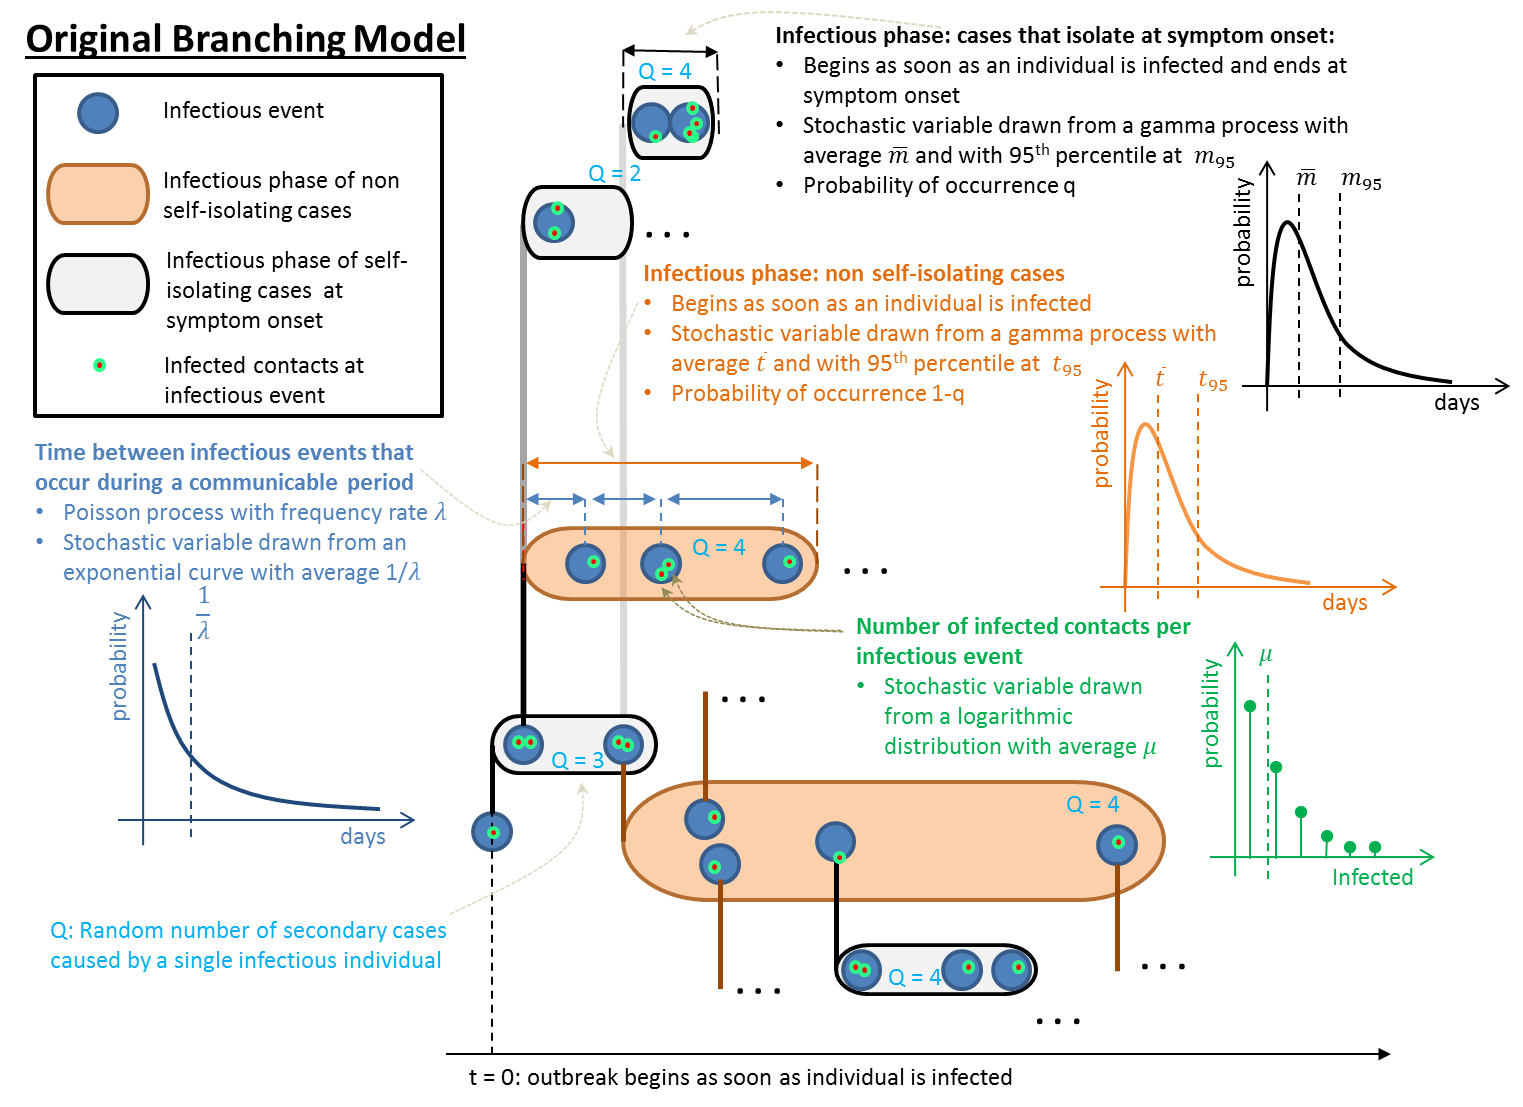
\includegraphics[width=0.99\textwidth, keepaspectratio=true]{figures/BranchingModel}
  \caption{Figure Title.}\label{fig_branchingModel}
\end{figure}


\subsection{Modified outbreak model}
[We added latent phase, the probability of infection, contacts, and testing.

we need to put modified \Rz, \Reff, branching \Reff\ somewhere in this section... 

The default parameters for the contacts and testing are listed in in Table \ref{table_defaultParams}. Although these must always be set, they are not relevant when only interested in the number of infected. ]

\begin{figure}
  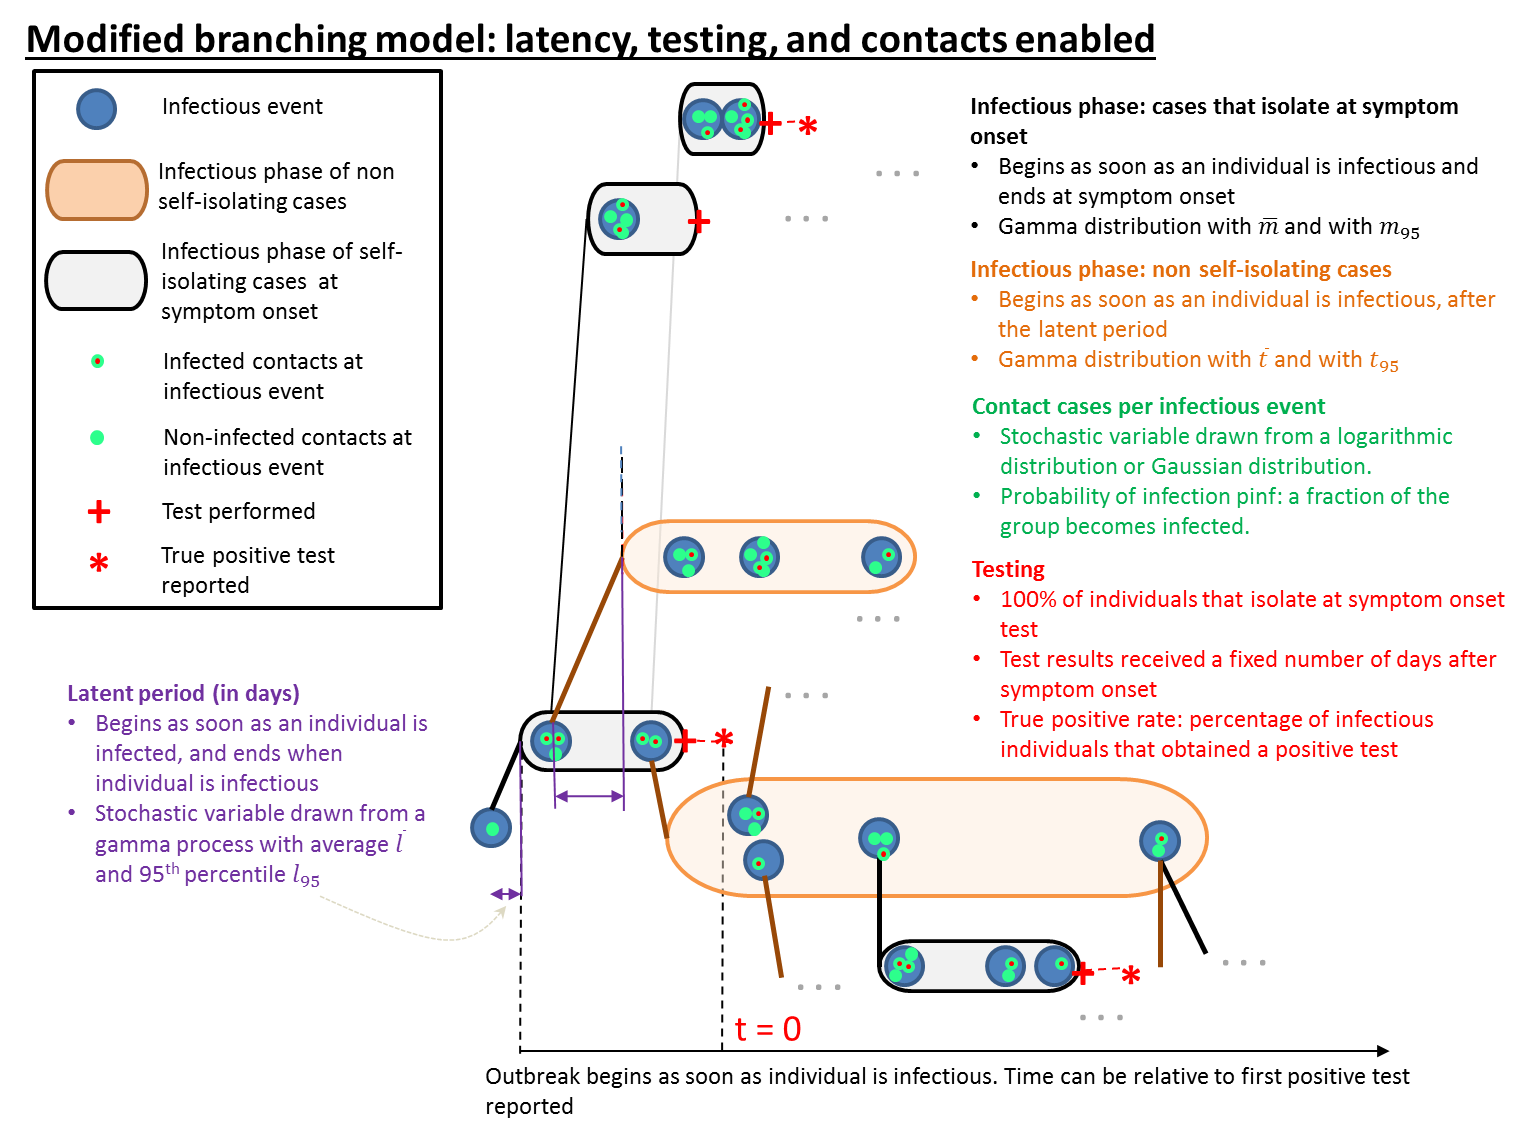
\includegraphics[width=0.99\textwidth, keepaspectratio=true]{figures/ModifiedBranchingModel}
  \caption{Figure Title.}\label{fig_branchingModel}
\end{figure}

\subsubsection{Effective reproduction number for a modified branching process}
As in the transmission branching model \cite{branchsim}, a compound Poisson process with arrival rate $\lambda$ and of duration $t$ is defined, with $Q(\lambda t)$ expressed as
\begin{equation}
Q(\lambda t)=\sum_{i=1}^{N(\lambda t)}Y_i,
\end{equation}
where $N(\lambda t)\sim\Pois(\lambda t)$ is the number of events from the Poisson process.
The PMF for $Q(\lambda t)$, is written as $P_{Q(\lambda t)}(q)$.
The compound Poisson process is then subordinated with a gamma process which has the PDF
\begin{equation}
f_{T(a,b)}(t)=\frac{b^a}{\Gamma(a)}t^{a-1}e^{-bt}\label{gammaPDF}
\end{equation}
and a mean of $\bar{t}=a/b$.
If $Z(\lambda,a,b)\equiv Q(\lambda T(a,b))$ is defined as the number of new infections from the subordinated Poisson process, where the duration $t$ from the Poisson process has been smeared by the gamma process with parameters $a$ and $b$, the PMF for $Z$ is given by
\begin{align}
P_{Z(\lambda,a,b)}(z) & = \int_0^\infty P_{Z(\lambda,a,b),T(a,b)}(z,t')dt'\nonumber\\
& = \int_0^\infty P_{Z(\lambda,a,b)|T(a,b)=t'}(z)f_{T(a,b)}(t')dt'\nonumber\\
& = \int_0^\infty P_{Q(\lambda t')}(z)f_{T(a,b)}(t')dt'.
\end{align}
The characteristic function for $Z(\lambda,a,b)$ can thus be expressed as
\begin{align}
\ex{e^{iuZ(\lambda,a,b)}} & = \sum_z e^{iuz}P_{Z(\lambda,a,b)}(z)\nonumber\\
& = \int_0^\infty \sum_z e^{iuz}P_{Q(\lambda t')}(z)f_{T(a,b)}(t')dt\nonumber\\
& = \int_0^\infty \ex{e^{iuQ(\lambda t')}}f_{T(a,b)}(t')dt'.\label{ZCF}
\end{align}

The PMF for $Q(\lambda t)$ can be written as
\begin{equation}
P_{Q(\lambda t)}(q) = \sum_n P_{Q(\lambda t)|N(\lambda t)=n}(q)P_{N(\lambda t)}(n),
\end{equation}
such that its characteristic function, assuming independent and identically-dis\-tri\-bu\-ted $Y_1,Y_2,\ldots Y_n$ variables, is given by
\begin{align}
\ex{e^{iuQ(\lambda t)}} & = \sum_q e^{iuq}P_{Q(\lambda t)}(q)\nonumber\\
& = \sum_n \sum_q e^{iuq}P_{Q(\lambda t)|N(\lambda t)=n}(q)P_{N(\lambda t)}(n)\nonumber\\
& = \sum_n \sum_{Y_1}\ldots\sum_{Y_n} e^{iu\sum_{i=1}^nY_i}P_{Y_1,\ldots,Y_n}(y_1,\ldots,y_n)P_{N(\lambda t)}(n)\nonumber\\
& = \sum_n \ex{e^{iuY}}^nP_{N(\lambda t)}(n)\nonumber\\
& = \sum_n \ex{e^{iuY}}^n\frac{e^{-\lambda t}(\lambda t)^n}{n!}\nonumber\\
& = e^{\lambda t\left(\ex{e^{iuY}}-1\right)}.\label{QCF}
\end{align}
Using Equations \eqref{gammaPDF}, \eqref{ZCF} and \eqref{QCF},
\begin{equation}
\ex{e^{iuZ(\lambda,a,b)}} = \left[1+\frac{\lambda}{b}\left(1-\ex{e^{iuY}}\right)\right]^{-a}.
\end{equation}
The characteristic function of $Z(\lambda,a,b)$ is then used to compute the expected value and the variance of the resulting subordinated compound Poisson process:
\begin{align}
\ex{Z(\lambda,a,b)} & = \frac{\lambda a}{b}\ex{Y}\label{exz}\\
\var{Z(\lambda,a,b)} & = \left(\ex{Z(\lambda,a,b)}\right)^2\left\{\frac{1}{a} + \frac{1}{\ex{Z(\lambda,a,b)}}\frac{\ex{Y^2}}{\ex{Y}}\right\}.\label{exz2}
\end{align}

\subsubsection{Latent phase and time parameterisation}

\subsubsection{Model modifications beyond a branching process}
Infection interruption due to CT, constraints on the primary individual, \texttt{nimax}, \texttt{npostestmax}.

\subsection{Interrupted branching model}
This is a subsection.

Lockdown is an effective method at controlling the spread of the virus [REF]. The model was modified to support, and evaluate the impacts of, full lockdown... 

Lockdown is a drastic measure that has a negative impact on the economie and... [REF]. It has been shown that reducing the infectious phase helps control the spread of the virus [REF]. It is reported that contact tracing has for objective to shorten the infectious phase window by encouraging non-self-isolating individuals to self-isolate [REF]. 

Support for contact tracing and lockdown were added. 

\begin{figure}
  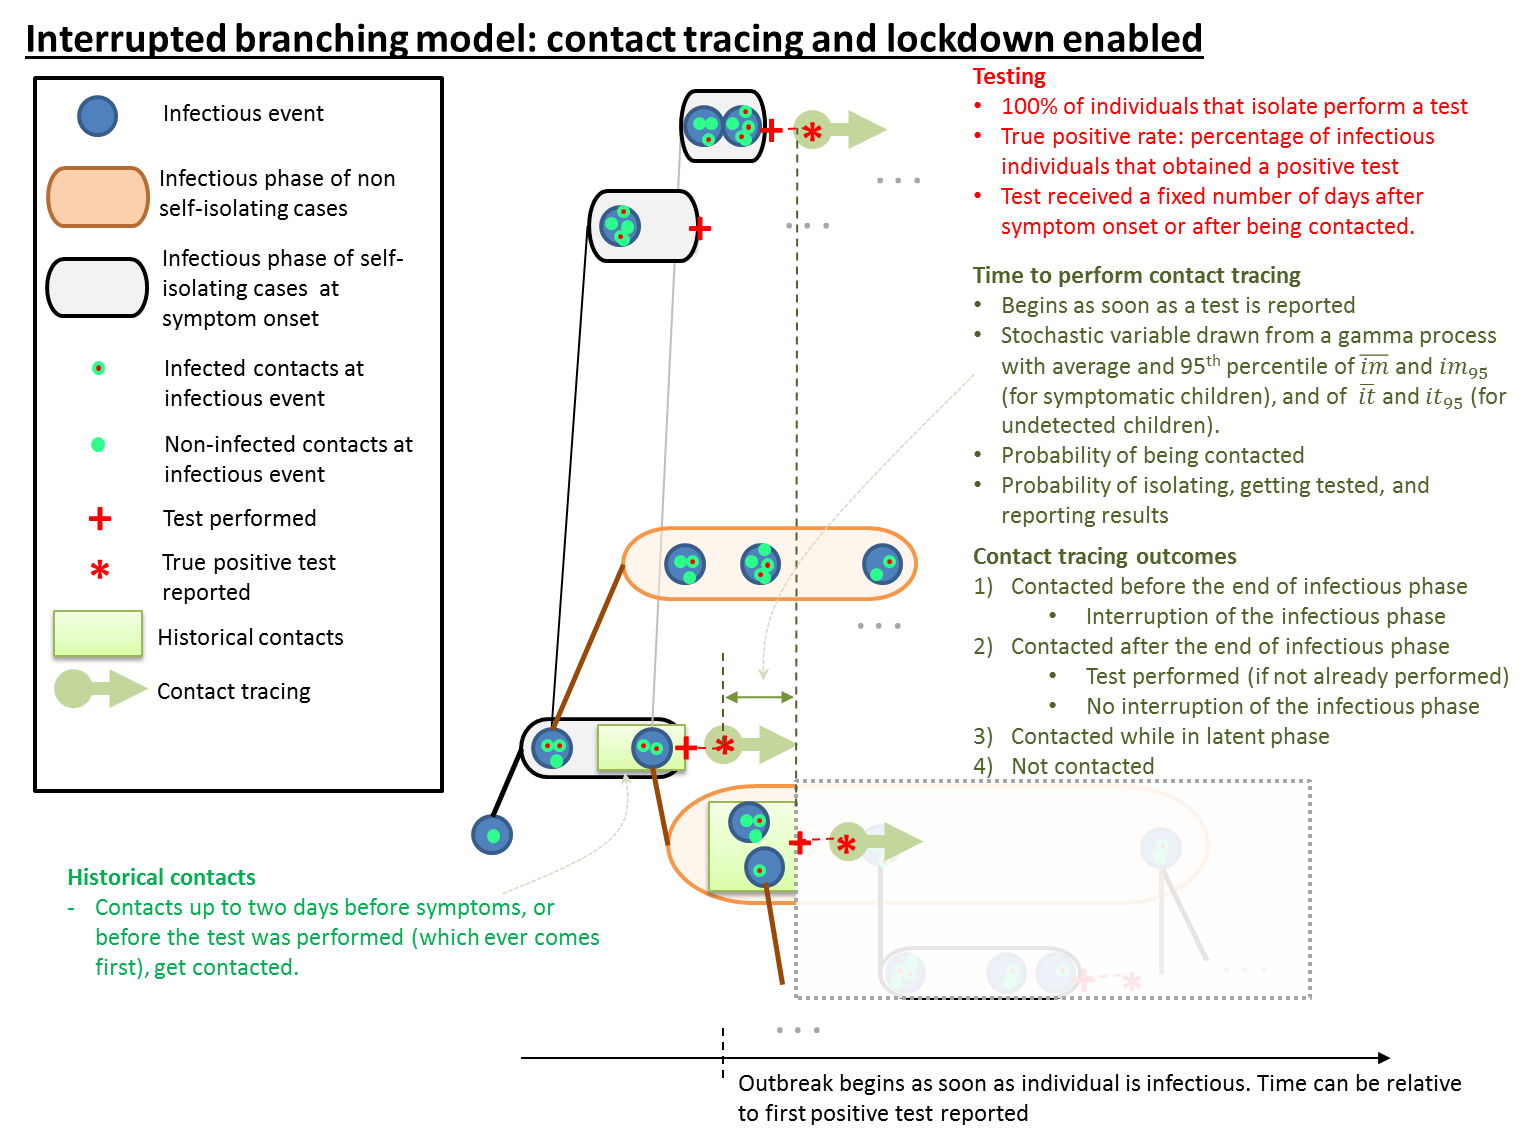
\includegraphics[width=0.99\textwidth, keepaspectratio=true]{figures/InterruptedBranchingModel}
  \caption{Figure Title.}\label{fig_branchingModel}
\end{figure}

\subsection{Summary of the interrupted branching model and its parameters}
This is a subsection.

From P-L email to Melanie...
The original model is a continuous time branching process of COVID-19 propagation based on a compound Poisson process of transmission event. The number of infections that occur at each event follows a logarithmic distribution. The Poisson process is subordinated by a random infectious period. The distribution for the random period can be itself randomly selected between two cases, each one represented by a different gamma distribution. There is no support for a latent period in the original model. There is no support for the generation of contacts and testing either, which are required to estimate contact tracing resources. The infectious periods cannot be truly interrupted through isolation in the original model, or at least in a way that is representative of how contact tracing is applied.

In the modified model, a latent period is introduced, which delays the start of the infectious period, post contamination. The propagation components required to estimate CT resources and to more correctly apply CT in the simulation have been added. The concept of probability of infections has been introduced, which is necessary to generate contacts, but that also allows to decouple interactions from contaminations, which produces a parameterisation that can be interpreted, but also be input much more easily. For scenarios where transmission occur through events where the number of interactions is not logarithmically distributed, other types of distributions can be used with the modified model. With the modified model it is also possible to look at observed infections (through positive test results), and to change the time reference when generating output distributions (e.g., time since the first positive test). In the modified model, there are options to select characteristics for the primary infectious individuals, and also to apply filters and cuts when generating results.

The model is different, but the implementation is also completely independent from the original model. The code of the modified model is about 1,000 faster than the one of the original model, and it supports parallel processing, which allows to generate far more statistics in the same amount of time.

\begin{table}
\centering
\caption{List of parameters and their default values (when applicable).}\label{table_defaultParams}
\begin{tabular}{p{6cm}ll}
Parameter & Designation & Default value\\
\hline
\hline
\multicolumn{3}{c}{Branching parameters} \\
Probability of infection & \Pinf & 1\%\\
Probability of self-isolating & $q$ & 0\%\\
\hline
\multicolumn{3}{c}{Testing parameters} \\
{\raggedright Test true positive rate\\for non-self-isolating individuals} & \ttpr & 70\%\\
{\raggedright Test true positive rate\\for self-isolating individuals} & \mtpr & 70\%\\
Testing delay & \tdeltat & 2 days\\
\hline
\multicolumn{3}{c}{Contact tracing parameters} \\
Probability of being contacted & \Pt & 80\%\\
Historical contact window & \ctwindow & 2 days\\
\hline
\end{tabular}
\end{table}


\section{Assumptions and parameters about the infectious disease}\label{Assumptions_section_label}

The following assumptions about the infectious disease, summarized in Table \ref{table_diseasePhase}, were considered:

\begin{itemize}
\item The incubation period of self isolating infectious individuals is drawn from a gamma distribution with a mean of 5.5 days and a \nfpc\ percentile of 9.72 days [Lauer et al...find ref].  
\item The infectious phase of self-isolating infectious individuals is drawn from a gamma distribution with mean of 2.2 days and a \nfpc\ percentile of 6.8 days [Zhao... find ref].
\item The latent phase was set as the difference between the self isolating individuals' incubation phase (5.5 days) and infectious phase (2.2 days); therefore, the mean was 3.3 days. To match the \nfpc\ percentile of the combined latent and infectious phases of self-isolating individuals with the \nfpc\ percentile of the non-self-isolating individuals' incubation phase as closely as possible, the \nfpc\ percentile of the latent phase was also set to 3.3 days. Thus, the duration of the latent phase is assumed fixed.  
\item The infectious phase for non-self-isolating infectious individuals was based on assumptions in [REF to Steve and Ramzi’s calculator].
\end{itemize}

\begin{table}
\centering
\caption{Disease time period for self-isolating and non-self-isolating infected individuals used in this work.}\label{table_diseasePhase}
\begin{tabular}{lrrl}
& Gamma distribution {   } - &Estimate (\nfpc\ percentile)\\
\hline
\textbf{\underline{Infected type}} & \textbf{\underline{Latent phase}} & \textbf{\underline{infectious phase}}\\
\textbf{Self-isolating} & 3.3 (3.3) & 2.2 (6.8)\\
\textbf{Non-self-isolating} & 3.3 (3.3) & 6.79 (12.2)\\
\hline
\end{tabular}
\end{table}

The parameters listed in this section were used throughout this work, unless specified otherwise. 

%\section{Performance metrics --- maybe section...}

\section{Simulations I - Modified branching model: General evaluation of the impact of self-isolating, of group size, of frequency of event, and of probability of infection on the spread of the virus}\label{Scenario_I_section_label}

It is common for epidemiologist to use the basic or effective reproduction number (\Rz\ and \Reff, respectively) to measure the spread of a virus [REF]. It is well known that if the \Rz\ of a virus is bellow 1, outbreaks will go extinct. If $\Rz > 1$, measures to contain the spread of a virus need to be put in place. \Reff\ measures the spread of the virus once measures are in place, and if $\Reff < 1$ than the control measures are effective at preventing the spread of the outbreak. 

But what happens to outbreaks if \Rz\ and \Reff\ are greater than 1? Although the exact value of the COVID-19 \Rz\ is debatable [REF,REF...], it is consensus that its value is well above 1; therefore, measures need to be put in place to prevent the spread of the virus. 

According to branching theory, the average \Reff\ can be computed as in Equation (add link here). It is well known that self-isolating when infected with the COVID-19 virus limits the infectious phase, which helps control the spread of the virus [REF]. It is also known that the group size (represented by the average of the distribution $\mu$, in Equation (addl link)), frequency of infectious events ($\lambda$), and probability of infections (\Pinf) all impact the spread of the virus [REF]. Figure \ref{fig_plt_brReffvsq} shows the value of \Reff\ for different values of probability of self-isolating ($q$) and of $\mu\lambda\Pinf$. From this figure, it is noticeable that as the probability of self-isolating ($q$) increases, $\mu\lambda\Pinf$ can be relaxed (i.e., increased) for a given \Reff\ value. 

As mentioned, for all outbreaks to become extinct the \Reff\ must be smaller than 1, but for larger values of \Reff, some outbreaks may also become extinct. The probability of extinction, defined as the number of outbreaks that are extinct overall outbreaks, captures the chances that outbreaks go extinct for $\Reff > 1$. As \Reff\ increases, the probability of extinction may, or may not decrease, as it is dependent on the various factors previously mentioned ($\mu$, $\lambda$, \Pinf\, etc.). To help make decisions, it is important for health officials to understand the impact that these various factors have on the probability of extinction when $\Reff > 1$. 

Using the branching model, this section shows the impact of varying $\mu$, $\lambda$, and \Pinf\ on the probability for extinction for specific values of \Reff, $q$, and  $\mu\lambda\Pinf$. These specific values are illustrated by a star marker in Figure \ref{fig_plt_brReffvsq}, where $\Reff = 2.018$ and $\Reff = 1.009$. These were selected as the literature reports that 60\% of individuals self-isolate when symptomatic [REF], and several have reported that, on average, one individual infected with COVID-19 will infect 2 others [REF]. The $\Reff = 1.009$ was evaluated for comparison purposes.
 
\subsection{Methodology, assumptions, and parameters} 

The simulations in this section had disease parameters listed in Table \ref{table_diseasePhase}, and had a q = 0.6.  

Two categories of simulations, with different $\mu\lambda\Pinf$ value, were performed. The values of $\mu\lambda\Pinf$ evaluated were 0.25 and 0.5, each of which having an \Reff\ of 1.009 and 2.018, as illustrated in Figure \ref{fig_plt_brReffvsq}. For each of the values evaluated, the \Pinf\ was either 0.125 or 1, and the $\mu$ value was 1, 2, 4, 8, 16, or 32. The $\lambda$ value was selected to satisfy the $\mu\lambda\Pinf$ as illustrated in Figure \ref{fig_plt_muvslambda}. This resulted in a total of 24 different simulations listed in Table \label{table_simIparams}. For all, the group was assumed to be drawn for a log plus 1 distribution with $\mu$. 

Each simulation were ran for 60 days on 10,000 outbreaks. The following performance metrics were evaluated:

\begin{enumerate}
\item The total number of infected over the 60 days averaged across the 10,000 outbreaks;
\item The probability of extinction, which is defined as the number of outbreaks that go extinct overall the outbreaks; and,
\item The average time of extinction, across all paths that went extinct. 
\end{enumerate}

Since the the beginning of an outbreak in real-time is unknown, the concept of time relative to the beginning of the outbreak is abstract; therefore, the time of extinction was computed relative to the first positive test reported. Testing parameters were set to the default values listed in Table \ref{table_defaultParams}. The simulations were also performed on observable paths only as those that are unobserved go extinct without any positive test reported. 

\begin{table}
\centering
\caption{Disease time period for self-isolating and non-self-isolating infected individuals used in this work.}\label{table_diseasePhase}
\begin{tabular}{lrrl}
& Gamma distribution {   } - &Estimate (\nfpc\ percentile)\\
\hline
\textbf{\underline{Infected type}} & \textbf{\underline{Latent phase}} & \textbf{\underline{infectious phase}}\\
\textbf{Self-isolating} & 3.3 (3.3) & 2.2 (6.8)\\
\textbf{Non-self-isolating} & 3.3 (3.3) & 6.79 (12.2)\\
\hline
\end{tabular}
\end{table}

\begin{table}
\centering
\caption{Parameter values used in simulations I.}\label{table_simIparams}
\begin{tabular}{lrrrrrr}
Sim Num. &	\Reff	& \Pinf &	$\mu$ &	$\lambda$ & $\mu\lambda\Pinf$	 & P-ext\\
\hline
1&	2.018&	0.1250&	1&	4	&0.50&0.3854\\
2	&2.018&	0.1250&	2&	2	&0.50&0.4088\\
3&	2.018&	0.1250&	4&	1	&0.50&0.4726\\
4&	2.018&	0.1250&	8&	0.5	&0.50&0.5831\\
5&	2.018&	0.1250&	16&	0.25&	0.50&0.7068\\
6&	2.018&	0.1250&	32	&0.125&	0.50&0.8219\\
7&	2.018&	1.0000&	1&	0.5	&0.50&0.3805\\
8&	2.018&	1.0000	&2&	0.25&	0.50&0.5523\\
9&	2.018&	1.0000	&4	&0.125&	0.50&0.7172\\
10&	2.018&	1.0000	&8	&0.0625	&0.50&0.8488\\
11&	2.018&	1.0000	&16	&0.03125&	0.50&0.9281\\
12&	2.018&	1.0000	&32	&0.015625&	0.50&0.964\\
\hline
13&	1.009&	0.1250&	1&	2&	0.25& 0.8672 \\
14&	1.009&	0.1250&	2&	1&	0.25&0.8756\\
15&	1.009&	0.1250&	4&	0.5&	0.25&0.9076\\
16&	1.009&	0.1250&	8&	0.25&	0.25&0.9325\\
17&	1.009&	0.1250&	16&	0.125&	0.25&0.9559 \\
18&	1.009&	0.1250&	32&	0.0625&	0.25&0.9772\\
19&	1.009&	1.0000&	1&	0.25&	0.25&0.8679\\
20&	1.009&	1.0000&	2&	0.125&	0.25&0.9256\\
21&	1.009&	1.0000&	4&	0.0625&	0.25&0.962\\
22&	1.009&	1.0000&	8&	0.03125&	0.25&0.9825\\
23&	1.009&	1.0000&	16&	0.015625&	0.25&0.9902\\
24&	1.009&	1.0000&	32	&0.00781250&	0.25&0.9964\\
\hline
\end{tabular}
\end{table}


\subsection{Results}
Results for the probability of extinction, time of extinction, and total number of infected as $\mu$ and $\lambda$ increase for the simulations listed in Table \ref{table_simIparams} are illustrated in Figure \ref{fig_plt_pextExp1}, Figure \ref{fig_plt_textExp1}, and Figure \ref{fig_plt_NinfExp1} respectively.


Figure \ref{fig_plt_pextExp1} shows that simulations with $\Reff = 1.009$ (the orange and blue markers) obtained highest probability of extinction on 10,000 observable outbreaks. The figure also shows that for increasing $\mu$ and decreasing $\lambda$, the probability of extinction increases. For a given \Reff, the simulations with highest \Pinf\ also obtained better p-ext. 


Figure \ref{fig_plt_textExp1} shows that simulations with smaller $\Reff = 1.009$ (the orange and blue marker) take, extinct outbreaks took more time to reach extinction, this is especially true for increasing $\lambda$ and smaller $\mu$. With the exception of $\Reff = 2.018$ and $\Pinf = 0.125$ (green markers), increasing $\mu$ while reducing $\lambda$ reduced the time to extinction. Some simulations obtained negative extinction time, meaning that the extinct outbreaks occurred, on average, before the first positive test was received.  


Figure \ref{fig_plt_NinfExp1} shows that simulations with $\Reff = 1.009$ had fewer infected individuals averaged overall 10,000 observable outbreaks after 60 days. Simulations with larger $\mu$ and \Pinf\ also had a higher number of infected individuals average across 10,000 observable outbreaks. 


\subsection{Discussion of results}
The results from Figure \ref{fig_plt_pextExp1} show that reducing \Reff\ improves the probability of extinction, this is due to the fact that each infectious individual infect fewer people. For a given \Reff, the probability of extinction can be improved by reducing the frequency of infectious events. Reducing the frequency of events allows for larger group gatherings (for constant \Reff\ values) without negatively impacting the p-ext, however this could results in a larger number of infected individuals, as illustrated in Figure \ref{fig_plt_NinfExp1}. The average number of infected individual overall 10,000 observable outbreaks is high due to the the number of infected individual from non-extinct paths. This is illustrated in Figure \ref{fig_plt_NinfExtExp1} and Figure \ref{fig_plt_NinfOutExp1} where the average number of infected individual after 60 days are averaged across extinct, and non-extinct outbreaks, respectively.  

Figure \ref{fig_plt_pextExp1} also shows that, reducing the frequency of infectious events allows for larger \Pinf, explaining why the curves with highest \Pinf\ obtained better p-ext. In fact, for a given average group size and \Reff, reducing the frequency of events while increasing \Pinf\ improved p-ext. This was especially true for $\Reff = 2.018$. But, larger \Pinf\ could also have disastrous consequences: a population with a larger proportion of infected individuals as illustrated in Figure \ref{fig_plt_NinfExp1}.

Reducing the frequency of events increase the time to reach extinction as illustrated in Figure \ref{fig_plt_textExp1}. This is explained by the fact that infectious events are spread out in time, meaning that the last event will occur later in time. Events with large $\mu$ reduce the time of extinction as infections are likely to occur at the same moment; and, hence also end at the same moment. In some cases, outbreaks will go extinct before the first positive test case is received. Unless $\Reff < 1$, this is undesirable as it does not allow health authorities enough time to react to the outbreak; by the time a test results is received, the outcome of the outbreak has already past, and if the outbreak is not extinct, it has already gone out of control. High values of $\mu$ and \Pinf\ drive the extinction time down. This can be explained by the fact that a larger number of people are getting infected in any single infectious event, rather than infections occurring more spread out in time. This can be undesirable as it does not allow health official enough time to react to non-extinct paths. 

\subsection{Conclusions}

The probability of extinction (for $\Reff > 1$) is not linearly proportional to \Reff\ as it depends on $\mu$, $\lambda$ and \Pinf. Therefore, \Reff\ alone (if above 1) is an insufficient metric to describe the spread of a virus. Several factors not only impact \Reff\ and p-ext, but also the time of extinction, and the total number of infected individuals. There are all important measures to help describe the spread of the virus. 

The results suggest that having a low frequency of infectious events prevents the spread of the disease and, in the context of the disease parameters selected (Table \ref{table_diseasePhase}), is the most effective course of action to control an outbreak. Although it may increase the time for outbreaks to reach extinction, it also allows official more time to react and control the outbreak. If the reduction in the rate of infectious events is compensated by large groups, or by an increase in \Pinf (relaxing social distancing measure or not using NPIs, for example), the probability of extinction may not be impacted, but the high number of infected individuals in non-extinct outbreaks could have disastrous consequences. Reducing the group size and the probability of extinction not only reduces the total number of infected individuals, but it also allows authorities more time to observe outbreaks (via positive test reports of COVID-19) before it is too late.  

The best way to improve the probability of extinction is by reducing \Reff. This can be achieved various ways, and most importantly by increasing the percentage of infected people that self-isolate, as illustrated in Figure \ref{fig_plt_brReffvsq}. When people self-isolate, they reduce their chances of infected others by reducing their infectious time window. Unfortunately, as reported in the literature [REF], not all infectious individuals that contract the COVID-19 virus have symptoms indicating to them that they should self-isolate. It is anticipated that other measures, such as contact tracing and isolating individuals that are contacted could help control the spread of the virus. 

The next Section evaluates the impact of different mitigation strategies in the context of the Diamond Princess outbreak. 

\begin{figure}
  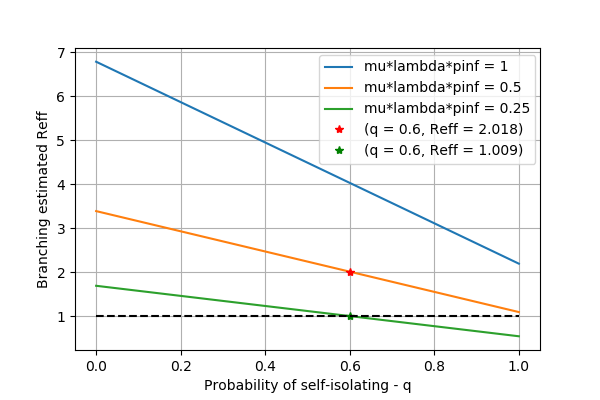
\includegraphics[width=0.99\textwidth, keepaspectratio=true]{figures/plt_brReffvsq}
  \caption{The branching model's estimated \Reff as the probability of self-isolating ($q$) increased so fixed values of $\mu\lambda\Pinf$ = 1, 0.5, and 0.25.}\label{fig_plt_brReffvsq}
\end{figure}


\begin{figure}
  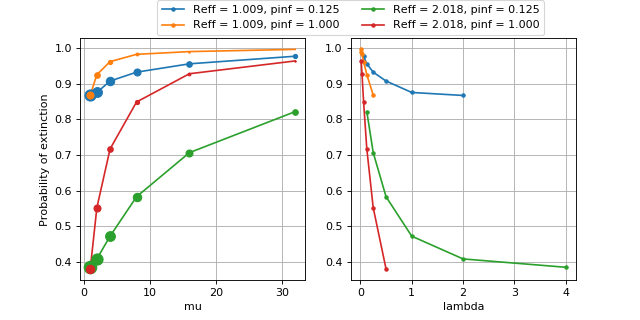
\includegraphics[width=0.99\textwidth, keepaspectratio=true]{figures/pext_exp1}
  \caption{Probability of extinction as a function of $\mu$ (left plot) and $\lambda$ (right plot). Increasing marker size indicates larger $\lambda$ (left plot).}\label{fig_plt_pextExp1}
\end{figure}

\begin{figure}
  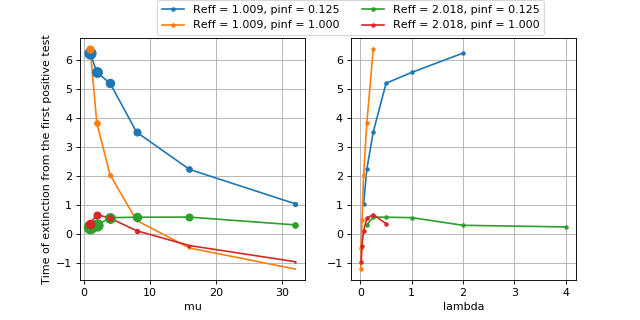
\includegraphics[width=0.99\textwidth, keepaspectratio=true]{figures/text_exp1}
  \caption{Time of extinction averaged across extinct outbreaks as a function of $\mu$ (left plot) and $\lambda$ (right plot). Increasing marker size indicates larger $\lambda$ (left plot).}\label{fig_plt_textExp1}
\end{figure}

\begin{figure}
  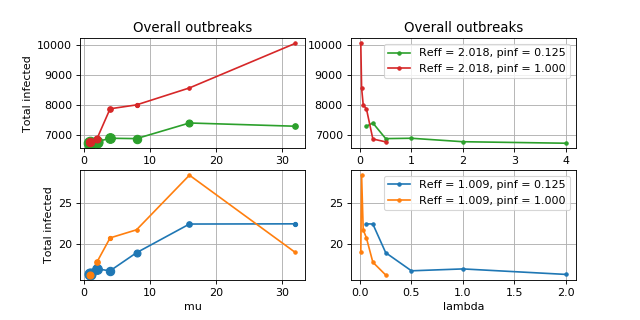
\includegraphics[width=0.99\textwidth, keepaspectratio=true]{figures/Ninf_exp1}
  \caption{Total number of infected averaged across all outbreaks as a function of $\mu$ (left plots) and $\lambda$ (right plots). Increasing marker size indicates larger $\lambda$  (left plot).}\label{fig_plt_NinfExp1}
\end{figure}


\begin{figure}
  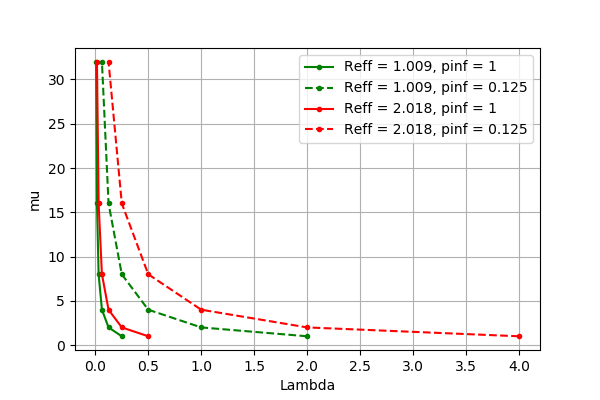
\includegraphics[width=0.99\textwidth, keepaspectratio=true]{figures/plt_muvslambda}
  \caption{Corresponding $\lambda$ values satisfying $\mu\lambda\Pinf$ for given $\mu$, \Pinf, and \Reff.}\label{fig_plt_muvslambda}
\end{figure}


\begin{figure}
  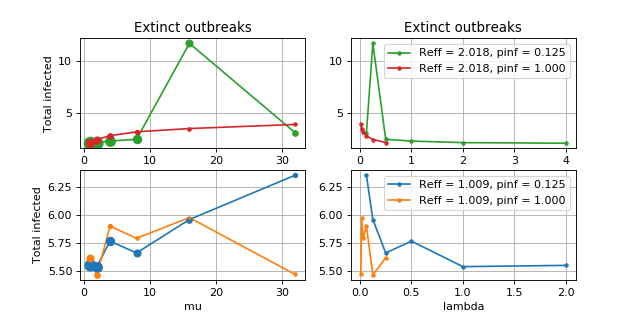
\includegraphics[width=0.99\textwidth, keepaspectratio=true]{figures/NinfExt_exp1}
  \caption{Total number of infected averaged across extinct outbreaks as a function of $\mu$ (left plots) and $\lambda$ (right plots). Increasing marker size indicates larger $\lambda$  (left plot).}\label{fig_plt_NinfExtExp1}
\end{figure}

\begin{figure}
  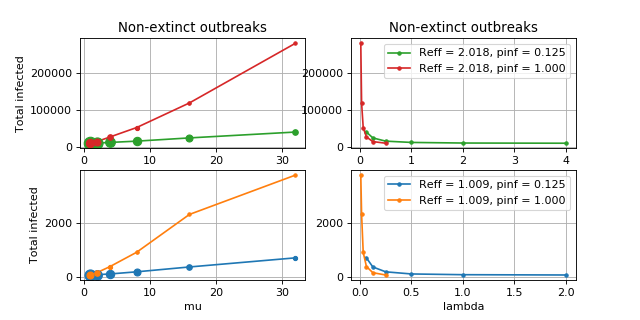
\includegraphics[width=0.99\textwidth, keepaspectratio=true]{figures/NinfOut_exp1}
  \caption{Total number of infected averaged across non-extinct outbreaks as a function of $\mu$ (left plots) and $\lambda$ (right plots). Increasing marker size indicates larger $\lambda$  (left plot).}\label{fig_plt_NinfOutExp1}
\end{figure}

\newpage

\section{Simulations II - Interrupted branching model: Scenario specific evaluation of the impact of different mitigation strategies}\label{Scenario_II_section_label}
This is a section.

\subsection{The Diamond Princess outbreak}

The Diamond Princess cruise ship departed Japan on January 20th 2020 \cite{10..15585/mmwr..mm6912e3}. On January 25th, the presumed primary infected individual left the ship. Some report that this individual was coughing before onboarding the ship \cite{10..1016/j..ijid..2020..02..033} while others report that coughing did not begin till the 23rd of January \cite{news_patient_zero}. This individual tested positive on February 1st, while on February 3rd the ship was quarantined from the rest of the world. Initial testing was performed on individuals with symptoms and their close contacts. Passengers were isolated from each other starting February 5th. Crew members, on the other hand, continued working, even if they had been in direct contact with a confirmed case. On February 4th, 10 COVID-19 cases were confirmed on-board the Diamond Princess.

Figure \ref{fig_chrono_DP}  (from \cite{10..15585/mmwr..mm6912e3}) illustrates the outbreak's chronology of events as well as the number of reported cases to the WHO. By definition, a reported case is a “person with laboratory confirmation of COVID-19 infection, irrespective of clinical signs and symptoms” \cite{WHO_surv}. 

There were a total of 2666 passengers and 1045 crew members (for a total of 3711 people) onboard the Diamond Princess \cite{10..15585/mmwr..mm6912e3}. A total of 706 were confirmed cases.  

There are reports that mitigation strategies to control the spread of COVID-19 on the Diamond Princess were not properly executed \cite{10..1002/jgf2..326}. Although the ship was quarantined 3 days after the primary individual reported positive to COVID-19, and, although contact tracing was executed on the ship to help control the outbreak among those on-board, it has been reported that the following may have contributed to the spread of the virus:

\begin{itemize} 
\item The suspected primary individual did not self-isolated on board of the Diamond Princess, even if he/she may have had symptoms while on the ship \cite{news_patient_zero}\cite{10..1016/j..ijid..2020..02..033};
\item Crew members that were in direct contact with a confirmed case did not self-isolate \cite{10..1002/jgf2..326} \cite{10..15585/mmwr..mm6912e3}; and,
\item A red-zone with proper decontamination was not set into place \cite{10..1002/jgf2..326}. 
\end{itemize}	
 
This section illustrates the use of the interrupted branching model to evaluate the impact of mitigating the concerns listed above on the Diamond Princess outbreak. The following are to be met:

\begin{enumerate}
\item Model the outbreak that occurred on the Diamond Princess using a modified branching model;
\item Demonstrate the impact of isolating the primary individual, of isolating all passengers and crew members that were in contact with an infected individual, and of minimizing the risk (or probability) of infection; and, 
\item Demonstrate the impact of the outbreak if no measures would have been set into place.
\end{enumerate}

\subsubsection{Methodology, assumptions, and parameters}

The simulations in this section had disease parameters listed in Table \ref{table_diseasePhase}, and had a q = 0.6. 

Although mitigation strategies were applied to the Diamond Princess, the outbreak had already begun once the first positive test case was reported. Therefore, the parameters that represent the social dynamics of the individuals on the ship were set to represent normal interaction before mitigation strategies were set in place. 

The average number of passengers per cabin was reported to be 1.98, whereas the average number of crew member was reported to be 1.73 \cite{10..15585/mmwr..mm6912e3}. It was assumed that people traveled as couples (i.e., in pairs of 2). However, the average group size at infectious events was 5 (therefore $\mu$ = 4), as it was assumed that couples congregated, and that at meal times congregated couples were served by at least one crew member. It was assumed that there were 4 infectious events per day (breakfast, lunch, diner, and one other event that could either be when an infected individual goes to bed, attends the gym, or attends a social event). Since passengers can attend various events on the Diamond Princess, and that there are several dining rooms, and exercise rooms, the group distribution was assumed log to allow for large group gatherings. 

The probability of infection at each infectious event was set to be 7\% (i.e., $\Pinf = 0.07$). This value was selected, because on February 4th, 10 days from when the primary individual left the diamond princess, 10 people were confirmed positive. These ten cases were assumed to have resulted from the same outbreak, therefore it can be assumed that during 9 days prior, an average of 1.11 individuals were infected per day. At 4 events per day, this results in 0.27 infected individuals per event (i.e., 10 infected / 9 days / 4 events per day = 0.27 infected per event). Since the distribution $\mu$ = 4, it was assumed that at each infectious event, 0.07 of the population was infected (i.e., 0.27 infected / 4  = 0.0675).

Since testing was performed in a controlled environment, it was assumed 0 days in testing delay, and 100\% true positive test rate for all those who tested (symptomatic and their contacts, symptomatic or not, tested). Since health authorities began isolating individuals after they received the first confirmed test, but that the primary individual had already left the ship, the time was set relative to the end of the primary individuals communicable period, which in this case is analogous to when the primary individual got off the ship. 

It was also assumed that on a ship, the probability of successful contact tracing was 1.0, and that the contact tracing window was short (0.5 days). The historic window of contacts was set to 5 days, meaning that on such a controlled setting, it was anticipated that those who tested positive were able to recall who they had been in contact with over the last 5 days. Asymptomatic crew members were not self-isolating even if they had been in contact with a positive case; therefore, the probability that non-self-isolating individual get contact traced and isolates was set to the ratio of passengers to total number of people on board (i.e., $\Pit = 2666/3711 = 0.72$).  All individuals that were symptomatic and that were in contact with a positive case self-isolated, either once contacted, or once symptoms appears (which ever occurred first). Since there is no mention of the primary individual self-isolating while on the Diamond Princess, if was assumed that the primary individual was non-self isolating. 

The parameters of the Diamond Princess outbreak are summarized in Table \ref{table_DPparams}, and are referred to as the \textit{baseline simulation}. 

From this baseline simulation, referred to as Sim0, some parameters were modified to simulate the following 5 scenarios and/or mitigation strategies:
\begin{enumerate}
\item Isolating all individuals (not just passengers) that were in direct contact with a confirmed cases. That is the probability that non-self-isolating individual get contact traced and isolate was set to 100\% (i.e., $\Pit = 1.0$). This simulation is referred to as Sim1;
\item Minimizing the probability of infection. Although it is unclear how masks, decontamination, or social distancing impacts the probability of infection, it was assumed that having a red-zone with proper decontamination would reduce the probability of infection by half, that is $\Pinf = 0.035$. This simulation is referred to as Sim2;
\item Self-isolation of the primary individual as soon as he/she had symptoms.This simulation is referred to as Sim3;
\item No contact tracing at the beginning of, and throughout the outbreak.This simulation is referred to as Sim4;
\item No contact tracing at the beginning of, and throughout the outbreak, but the primary individual self-isolated as soon as he/she had symptoms. This simulation is referred to as Sim5. 
\end{enumerate}

All simulations were performed on 10,000 outbreaks over 30 days. The parameters for all the above simulations are summarized in Table \ref{table_DPparams} and their appellation are summarized in Table \ref{table_DPsimsNames}. The parameters that differ from the baseline are in bold font.  

For each simulations, the average number of confirmed cases (i.e., positively reported tests) across all outbreaks was computed over time as well as the average number of infections over time. The probability of extinction, the time of extinction, and the distribution of the average number of infected was also computed. 

Since the statistics in the branching model cannot be changed over time, the model assumes that symptomatic individuals self-isolated from the beginning, and that contact tracing was initiated as soon as the outbreak began. Since this may not be the case, the model cannot be used as an absolute estimate, but rather as a relative study to evaluate the impacts of the various mitigation strategies. 

\subsubsection{Results}
The probability of extinction as well as the time of extinction for each simulation are listed in Table \ref{table_DPextResults}. These results show that Sim3 obtained highest probability of extinction followed by Sim5 and then Sim2. Sim4 obtained lowest probability of extinction. Extinct outbreaks reached extinctions within 0.456 and 5.389 days on average from the end of the primary's individual infectious phase. 

The total number of confirmed cases overtime is illustrated in Figure \ref{fig_DP_posTest}. These results show that the baseline simulation (Sim0) follows the real number of confirmed cases obtained from the WHO. It is also worth mentioning that the \Reff\ for the baseline simulation is 3.57, which closely matches \Rz\ values estimated at the beginning of the outbreak in China [REF]. Sim2 has the slowest rate of reported cases, however Sim3 have fewer reported cases up to 18 days where the number of reported cases start growing exponentially. Sim0, Sim1, and Sim4 have a comparable number of reported case, however Sim4 has fewer reported cases in the first 15 days. 

The total number of infected overtime is illustrate in Figure \ref{fig_DP_numInf}, and the total number of infected overtime for non-extinct path is illustrate in Figure \ref{fig_DP_numInfOut}. In both figures, the results show that Sim4 obtained the highest numbers of infected individuals and the fastest rate of infected. Sim5 is shifted from Sim4 in time. Sim3 and Sim0 are also shifted in time from each other. The results also show that Sim2 obtained the slowest rate of infected. However, in Figure \ref{fig_DP_numInf} Sim3 had the least number of infected in the first 15 days. 

Figure \ref{fig_DP_distReff}  shows the distribution of the number of secondary infections. The distribution is relative to the total number of infected overall outbreaks for a given simulation. This is to account for the fact that some simulations obtained a noticeably larger amount of infected individuals. For clarity, relative counts bellow 0.1\% aren't shown. The results show a peak in infected with 0 secondary infections; that is, between 47\% (Sim0, Sim12 and Sim3) and 54\% (Sim1) of infected individuals did not infect others. For Sim4 and Sim5, 20\% of infected did not infect others. The cumulative sum of this distribution (shown in Figure \ref{fig_DP_cumDistReff}) illustrates that for Sim2 close to 0\% of the infected individuals infected more than 15 other people, whereas for the other simulations between 5\% and 8\% of the infected individuals infected more than 15 other people. 


\subsubsection{Discussion of results}

The results from Table \ref{table_DPextResults} demonstrate that the probability of the outbreak going extinct within 30 days would have increased by 70\% if the primary individual infected that boarded the Diamond Princess would have self-isolated once symptoms appeared. Self-isolation alone (Sim5) without the measures taken on the Diamond Princess during the outbreak would have also improved the probability of extinction. These results suggest that, in this scenario, the infectious phase of the primary individual had a dramatic impact on the probability of extinction. It is interesting to note that extinction, if it were to occur, would have occurred rapidly or would have been unnoticeable (i.e., before a positive test was received) as extinction on averaged occurred in half a day from the end of the primary individuals infectious phase.

Although self-isolation of the primary individual increases the likelihood of extinction, this control measure does not necessarily suppress the total number of infected in non-extinct outbreaks. This will only shift the outbreak in time as it reduced the number of infections at the beginning of an outbreak, explaining the shift in time between Sim0 (baseline without primary individual self-isolating) and Sim3 (baseline with primary individual self-isolating), and between Sim4 (no control measure) and Sim5 (primary individual self-isolating only) in Figure \ref{fig_DP_numInf} and Figure \ref{fig_DP_numInfOut}. This measure will have very little impact on the outbreak overtime. In fact, self-isolating the primary individual will have no impact on the number of secondary infections as shown in Figure \ref{fig_DP_distReff} and Figure \ref{fig_DP_cumDistReff} where Sim0 and Sim3, and Sim4 and Sim5 have the same distribution in the secondary number of infected. These results suggest that the outbreaks are the same, but shifted in time. Such a time shift could have given authorities more time to better respond to the outbreak, but additional measures would have been required to mitigate the number of infected. 

Proper contact tracing of passengers and crew members, as in Sim1, increases the number of individuals that don't infect others (i.e., infectious non-spreading individuals), as demonstrated in Figure \ref{fig_DP_cumDistReff} where Sim1 obtained 54\% of individuals with 0 secondary infections, compared to 20\% for simulations without contact tracing (i.e., Sim4 and Sim5). Contact tracing will start to reduce the number of infected in non-extinct outbreaks 5 days after the end of the primary's individual communicable period, as illustrated in Figure \ref{fig_DP_numInfOut} (when comparing Sim1 to Sim4). However, it has little impact on the initial stages of the outbreak, and by the time the benefits of contact tracing are observed, there are already several infected individuals. In reality, contact tracing efforts may become less productive as more resources are required as the number of infected increases. This is contrary to the modeling that assumed that the contact tracing efforts were constant throughout the outbreak. This suggests that contact tracing alone was not a successful mitigation strategy for the outbreak that occurred on the Diamond Princess. Additionally, when comparing Sim1 to Sim5 in Figure \ref{fig_DP_numInfOut}, it is noticeable that, at the initial stages of the outbreak self-isolation of the primary individual will help minimize the number of infected more efficiently than proper contact tracing. 

Reducing the probability of infection, as in Sim2, noticeably reduces the number of infected in non-extinct outbreaks (Figure \ref{fig_DP_numInfOut}). This can be explained by the fact that there are fewer infected individuals that infect more than 15 others, as noticed in Figure \ref{fig_DP_distReff} and Figure \ref{fig_DP_cumDistReff}. From these figures, it is interesting to note that reducing the probability of infection (Sim2) had no noticeable impact on the number of individuals with 0 secondary infections. This suggest that reducing the number of super spreaders, rather then increasing the number of infectious non-spreading individuals, could have helped mitigate the number of infected in the Diamond Princess outbreak. Although reducing the probability of infection only provided 18\% probability of extinction (Table \ref{table_DPextResults}) after 30 days, the average number of days to extinction had a large variation (5.996), suggesting that increasing the simulation time would increase both the probability of extinction, and the time of extinction. This is illustrated in Figure \ref{fig_DP_pextTime} and Figure \ref{fig_DP_textTime}. These results suggest that, reducing the probability of infection effectively improves the probability of extinction, but that it just takes longer to reach extinction because the outbreaks occur at a slower rate then the simulations where the primary individual self isolated (Sim3 which had highest probability of extinction \ref{table_DPextResults}). 

\subsubsection{Conclusion}
These results show that if the primary infected individual would have self-isolated, the outbreak's likelihood of going extinct (and un-noticed) would have increased from 3\% to 73\%. 

Contact tracing efforts increased the number of infectious non-spreading individuals, but the results suggests that preventing super-spreaders could have been the most effective method to mitigate the Diamond Princess outbreak. Super-spreaders can be prevented by reducing the probability of infections. This can be achieved by social distancing, by using NPIs, and by performing proper decontamination [REF].

\begin{figure}
  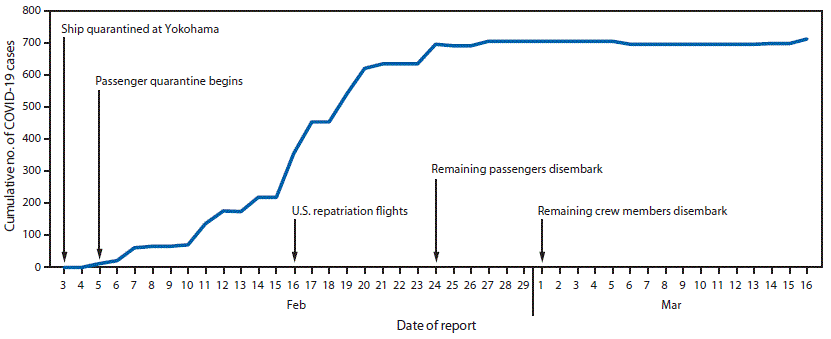
\includegraphics[width=0.99\textwidth, keepaspectratio=true]{figures/chrono_DP}
  \caption{Number of reported infected individuals on the Diamond Princess over the course of the outbreak along with marked events.}\label{fig_chrono_DP}
\end{figure}


\begin{table}
\centering
\caption{List of parameters for the Diamond princess simulations listed in Table \ref{table_DPsimsNames}.}\label{table_DPparams}
\begin{tabular}{p{3.8cm}p{1.5cm}|p{1.5cm}p{1.5cm}p{1.5cm}p{1.5cm}p{1.5cm}}
\hline
\textbf{Parameter} & \textbf{Baseline} & \textbf{Sim1} & \textbf{Sim2} & \textbf{Sim3} & \textbf{Sim4} & \textbf{Sim5} \\
\hline

$\mu$        		&	4		&	4		&	4			&4		&4				&4\\
$\lambda$		&	4		&	4		&	4			&4		&4				&4\\
\Pinf			&0.07		&	0.07	&\textbf{0.035}	&0.07	&0.07			&0.07\\			
\tdeltat		&	0		&	0		&	0			&0		&0				&0\\
\ttpr			&	1		&	1		&	1			&1		&1				&1\\
\mtpr		&	1		&	1		&	1			&1		&1				&1\\					
\Pt			&	1		&	1		&	1			&1		&1				&1\\
\ctwindow	&	5		&	5		&	5			&5		&5				&5\\
\Pit			&	0.72	&\textbf{1}	&	0.72		&0.72	&\textbf{0}		&\textbf{0}\\
\Pim			&	1		&	1		&	1			&1		&\textbf{0}		&\textbf{0}\\
\imbar, \itbar	&	0.5		&	0.5		&	0.5			&0.5	&\textbf{n-a}      &\textbf{n-a}\\		
\npaths		&	10000	&	10000	&	10000		&10000	&10000			&10000\\
\tmax		&	30		&	30		&	30			&30		&30				&30\\
\hline
\grouplog &  \checkmark   & \checkmark & \checkmark  & \checkmark & \checkmark  & \checkmark \\ 
\timerelpriendcomm &  \checkmark   & \checkmark & \checkmark  & \checkmark & \checkmark  & \checkmark \\ 
\observablepathsonly &  \checkmark   & \checkmark & \checkmark  & \checkmark & \checkmark  & \checkmark \\ 
\prinoaltperiod &  \checkmark   & \checkmark & \checkmark  &  & \checkmark  &  \\ 
\prinomainperiod &   &  &  &  \textbf{\checkmark} & &  \textbf{\checkmark} \\ 
\hline
\end{tabular}
\end{table}


\begin{table}
\centering
\caption{Appellation of the simulations.}\label{table_DPsimsNames}
\begin{tabular}{|p{1.5cm}p{10cm}|}
\hline
& \textbf{\underline{Simulation}}\\
 \textbf{Sim0} &Baseline\\
 \textbf{Sim1} &Contact tracing of both passengers and crew members in direct contact with a confirmed positive case\\
 \textbf{Sim2}  &Lowered probability of infection\\
 \textbf{Sim3}  &Primary self-isolated as symptoms appeared\\
 \textbf{Sim4}  &No contact tracing was performed at the beginning of the outbreak\\
 \textbf{Sim5}  &No contact tracing was performed at the begging of the outbreak, but the primary individual self-isolated\\
\hline
\end{tabular}
\end{table}

\begin{table}
\centering
\caption{Probability of extinction (after 30 days) and average time to extinction across all extinct outbreaks, for each simulation.}\label{table_DPextResults}
\begin{tabular}{p{4.7cm}|p{1.0cm}|p{1.2cm}p{1.2cm}p{1.2cm}p{1.2cm}p{1.2cm}}
\hline
\textbf{Metric} & \textbf{Sim0} & \textbf{Sim1} & \textbf{Sim2} & \textbf{Sim3} & \textbf{Sim4} & \textbf{Sim5} \\
\hline
Simulated \Reff & 3.575 & 3.101 & 2.000 & 3.567 & 5.527 & 5.525\\
Probability of extinction & 0.032 & 0.0664 & 0.1822 & 0.7278 & 0.0079 & 0.3695\\
Average days to extinction (+/-)* & 3.048 (3.407) & 4.653 (4.177) & 5.389 (5.996) & 0.573 (1.280)  & 1.400 (2.254) & 0.456 (1.456)\\
\hline
\multicolumn{7}{p{11.7cm}}{*Time is relative to the end of the primary individual's communicable period}\\
\end{tabular}
\end{table}

\begin{figure}
  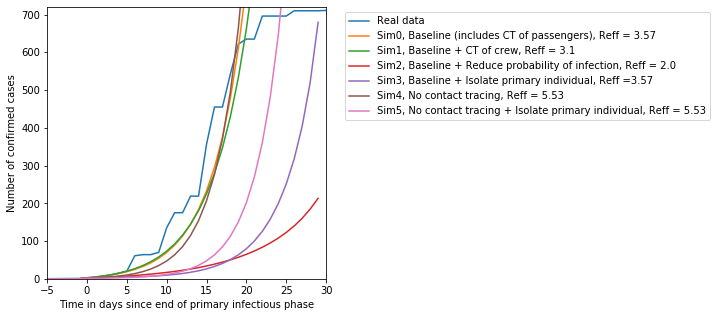
\includegraphics[width=0.99\textwidth, keepaspectratio=true]{figures/DP_posTest}
  \caption{Total number of confirmed cases over time averaged across all 10,000 observable outbreaks.}\label{fig_DP_posTest}
\end{figure}

\begin{figure}
  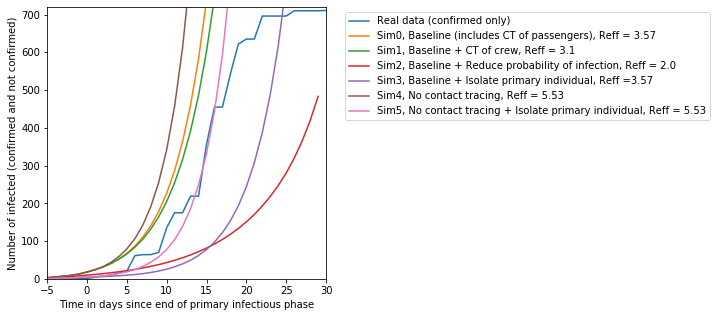
\includegraphics[width=0.99\textwidth, keepaspectratio=true]{figures/DP_numInf}
  \caption{Total number of infected over time averaged across all 10,000 observable outbreaks.}\label{fig_DP_numInf}
\end{figure}

\begin{figure}
  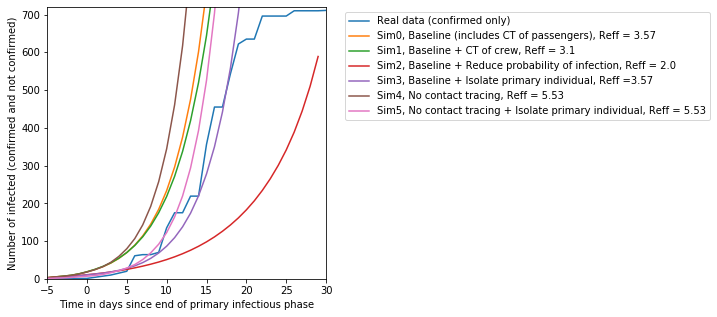
\includegraphics[width=0.99\textwidth, keepaspectratio=true]{figures/DP_numInfOut}
  \caption{Total number of infected over time averaged across all non-extinct and observable outbreaks.}\label{fig_DP_numInfOut}
\end{figure}

\begin{figure}
  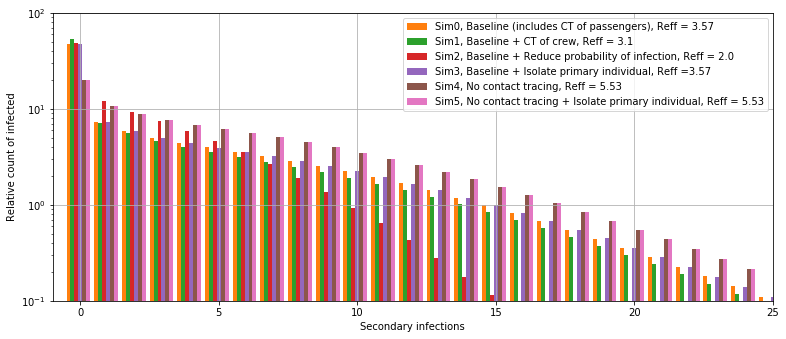
\includegraphics[width=0.99\textwidth, keepaspectratio=true]{figures/DP_distReff}
  \caption{The distribution of the number of the number of secondary infections caused by an infected person. The y-axis shows the log of the percentage of primary infected individuals between 0.1\% and 100\% across all the 10,000 outbreaks. The x-axis bins the number of secondary infected by integers from 0 to 25.}\label{fig_DP_distReff}
\end{figure}

\begin{figure}
  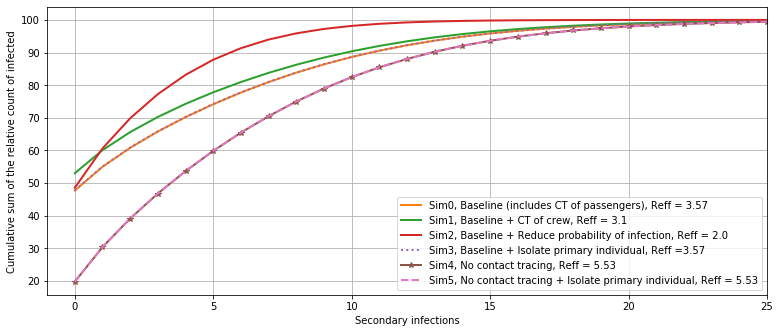
\includegraphics[width=0.99\textwidth, keepaspectratio=true]{figures/DP_cumDistReff}
  \caption{The cumulative sum of the number of infected causing secondary infections. The y-axis shows the log of the cumulative sum of infected individuals between across all the 10,000 outbreaks. The x-axis bins the number of secondary infected by integers from 0 to 25.}\label{fig_DP_cumDistReff}
\end{figure}

\begin{figure}
  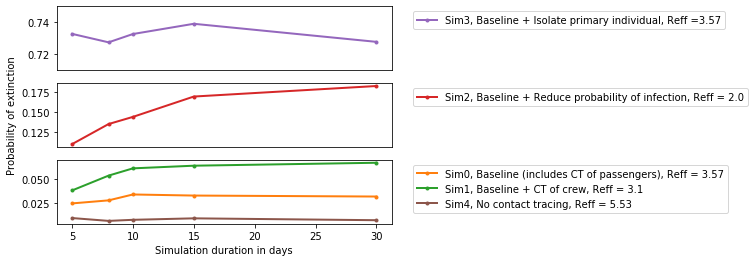
\includegraphics[width=0.99\textwidth, keepaspectratio=true]{figures/DP_pextTime}
  \caption{Probability of extinction for Sim2 as the simulation duration increases.}\label{fig_DP_pextTime}
\end{figure}

\begin{figure}
  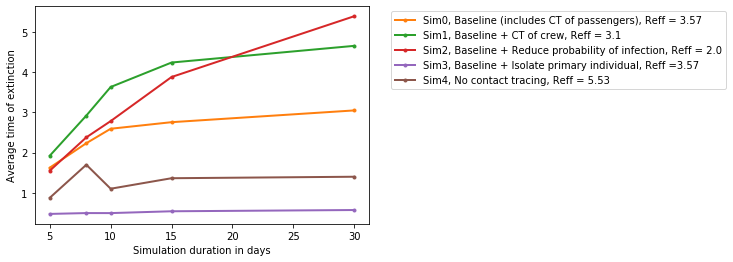
\includegraphics[width=0.99\textwidth, keepaspectratio=true]{figures/DP_textTime}
  \caption{Time of extinction for Sim2 as the simulation duration increases.}\label{fig_DP_textTime}
\end{figure}



\subsection{Tent scenario}
See BranchingForCT-20200929
\subsubsection{Assumptions and parameters}
\subsubsection{Methodology}
\subsubsection{Results}
\subsubsection{Discussion of results}


\subsection{Conclusions and discussion}

\section{Simulations III - Comparison to other models: CAF Ship Scenario}\label{Scenario_III_section_label}
\subsubsection{Assumptions and parameters}
\subsubsection{Methodology}
\subsubsection{Results}
\subsubsection{Discussion of results}

\section{Limitations of the interrupted branching model}\label{Limitations_section_label}
This is a section

\section{This model's application to the CAF}\label{CAF_Application_section_label}
This is a section.

As shown in Section \ref{first_section_label} on Page \pageref{first_section_label}.
According to \cite{archana_lucas_report}, \ldots

In Figure \ref{spectrum} and in Table \ref{table1}.

\begin{figure}
  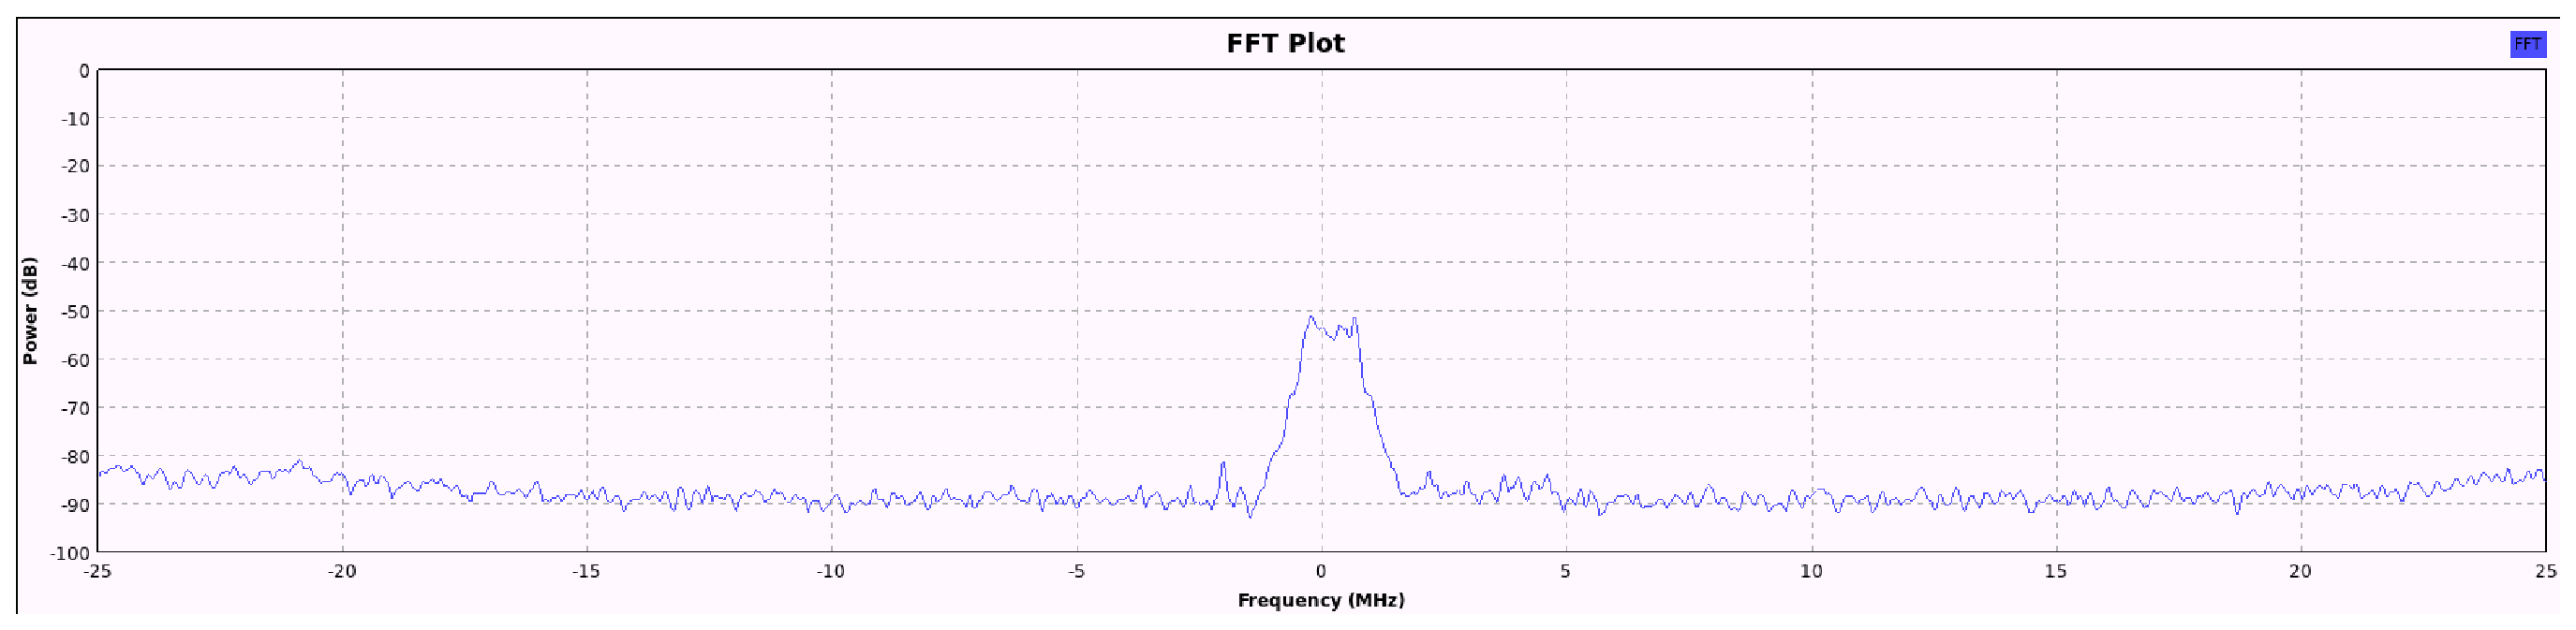
\includegraphics[width=0.99\textwidth, keepaspectratio=true]{figures/spectrum}
  \caption{Figure Title.}\label{spectrum}
\end{figure}

\clearpage

\begin{table}
\centering
\caption{My table.}\label{table2}
\begin{tabular}{lrrl}
Name & Value 1 \\
\hline
\hline
Name1 & 0 \\
Name2 & 8 \\
\hline
\end{tabular}
\end{table}


\section{Conclusions}\label{Conclusions_section_label}
Given the average social dynamics of the CAF scenario, what would be the chances of an outbreak not going extinct?

%\cleardoublepage
\bibliography{refs}
\bibliographystyle{drdc}

\docctl

%\makebackcover
\end{document}
